\documentclass[a4paper, 11pt,reqno]{article}
\input{macro/package.tex}
\input{macro/environement}
% Header et footer

\pagestyle{fancy}
\fancyhead{}
\fancyfoot{}
\renewcommand{\headwidth}{\textwidth}
\renewcommand{\footrulewidth}{0.4pt}
\renewcommand{\headrulewidth}{0pt}
\renewcommand{\footruleskip}{5px}

\fancyfoot[R]{Olivier Glorieux}
%\fancyfoot[R]{Jules Glorieux}

\fancyfoot[C]{ Page \thepage }
\fancyfoot[L]{1BIOA - Lycée Chaptal}
%\fancyfoot[L]{MP*-Lycée Chaptal}
%\fancyfoot[L]{Famille Lapin}

\input{macro/newcommand.tex}
\geometry{hmargin=1.0cm, vmargin=2.5cm}


\newcommand{\type}{TD }
\excludecomment{correction}
%\newcommand{\type}{Correction TD }

\begin{document}
\title{TD continuite}


\noindent\section{\large{\'Etude de la continuit\'e de fonctions num\'eriques}}


%-----------------------------------------------
\begin{exercice}  \;
	\'Etudier la continuit\'e des deux fonctions suivantes:
	$$
		f: x\mapsto (x^2-1)\sin{\left( \ddp\frac{1}{x-1} \right)}\qquad \hbox{et}\qquad g: x\mapsto \cos{(\ln{|x|})}\ln{(1+x)}.
	$$
\end{exercice}
\begin{correction}  \;
	\begin{enumerate}
		\item \textbf{\'Etudier la continuit\'e de la fonction suivante: $f: x\mapsto (x^2-1)\sin{\left( \ddp\frac{1}{x-1} \right)}$}\\
		      \begin{itemize}
			      \item[$\bullet$] Domaine de d\'efinition: La fonction $f$ est bien d\'efinie si $x-1\not= 0$. Ainsi $\mathcal{D}_f=\R\setminus\lbrace 1\rbrace$.
			      \item[$\bullet$] R\'egularit\'e: La fonction $f$ est continue sur $\mathcal{D}_f=\R\setminus\lbrace 1\rbrace$ comme somme, quotient, compos\'ee et produit de fonctions continues.
		      \end{itemize}
		\item \textbf{\'Etudier la continuit\'e de la fonction suivante: $g: x\mapsto \cos{(\ln{|x|})}\ln{(1+x)}$}\\
		      \begin{itemize}
			      \item[$\bullet$] Domaine de d\'efinition: la fonction $g$ est bien d\'efinie si $1+x>0$ et $|x|>0\Leftrightarrow x\not= 0$. Ainsi $\mathcal{D}_g=\rbrack -1,0\lbrack \cup \rbrack 0,+\infty\lbrack$.
			      \item[$\bullet$] R\'egularit\'e: La fonction $g$ est continue sur $\mathcal{D}_g=\rbrack -1,0\lbrack \cup \rbrack 0,+\infty\lbrack$ comme somme, compos\'ees et produit de fonctions continues.
		      \end{itemize}
	\end{enumerate}
\end{correction}


%-----------------------------------------------
\begin{exercice}  \;
	\'Etudier la continuit\'e des fonctions suivantes:
	\begin{enumerate}
		\begin{minipage}[t]{0.27\textwidth}
			\item $f(x)=\left\lbrace \begin{array}{ll}e^{-x}& \hbox{si}\ x>0\vsec\\ 0 &\hbox{sinon}  \end{array}\right.$
		\end{minipage}
		\begin{minipage}[t]{0.34\textwidth}
			\item $g(x)=\left\lbrace \begin{array}{ll} \ddp\frac{\ln{(1-4x)}}{2x}  & \hbox{si}\ x< 0\vsec\\ 1 &\hbox{si}\ x=0\vsec\\ \ddp\frac{e^x-1}{x} & \hbox{si}\ x>0  \end{array}\right.$
		\end{minipage}
		\begin{minipage}[t]{0.3\textwidth}
			\item $h(x)=\left\lbrace \begin{array}{ll} \ddp\frac{5x^2+4x}{1+x}  & \hbox{si}\ x< 0\vsec\\ 1 &\hbox{si}\ x=0\vsec\\ x\sin{\left( \ddp\frac{1}{x} \right)}& \hbox{si}\ x>0  \end{array}\right.$
		\end{minipage}
	\end{enumerate}
\end{exercice}
\begin{correction}  \;
	\begin{enumerate}
		\item \textbf{\'Etude de la continuit\'e de la fonction $f$ d\'efinie par $f(x)=\left\lbrace \begin{array}{ll}e^{-x}& \hbox{si}\ x>0\vsec\\ 0 &\hbox{sinon}  \end{array}\right.$:}
		      \begin{itemize}
			      \item[$\bullet$] Domaine de d\'efinition: $\mathcal{D}_f=\R^+$.
			      \item[$\bullet$] Continuit\'e sur $\R^{+\star}$: la fonction $f$ est continue sur $\R^{+\star}$ comme compos\'ee de fonctions continues.
			      \item[$\bullet$] Continuit\'e en 0: $\lim\limits_{x\to 0} f(x)=\lim\limits_{x\to 0} e^{-x}=1$ et $f(0)=0$. Ainsi $\lim\limits_{x\to 0} f(x)\not= f(0)$ et donc la fonction $f$ n'est pas continue en 0.
		      \end{itemize}
		      Conclusion: La fonction $f$ est continue sur $\R^{+\star}$ mais elle n'est pas continue en 0.
		      %--------
		\item \textbf{\'Etude de la continuit\'e de la fonction $g$ d\'efinie par $g(x)=\left\lbrace \begin{array}{ll} \ddp\frac{\ln{(1-4x)}}{2x}  & \hbox{si}\ x< 0\vsec\\ 1 &\hbox{si}\ x=0\vsec\\ \ddp\frac{e^x-1}{x} & \hbox{si}\ x>0  \end{array}\right.$:}
		      \begin{itemize}
			      \item[$\bullet$] Domaine de d\'efinition: si $x<0$, on a bien toujours $1-4x>0$ et $2x\not= 0$. De m\^{e}me, si $x>0$, on a bien toujours $x\not= 0$. Ainsi $\mathcal{D}_g=\R$.
			      \item[$\bullet$] Continuit\'e sur $\R^{\star}$: La fonction $g$ est continue sur $\R^{+\star}$ comme somme et quotient de fonctions continues et sur $\R^{-\star}$ comme somme, compos\'ee et quotient de fonctions continues. Ainsi elle est continue sur $\R^{\star}$.
			      \item[$\bullet$] Continuit\'e en 0:
			            \begin{itemize}
				            \item[$\star$] Par substitution, on a: $\ln{(1-4x)}\underset{0}{\thicksim} -4x$ et par quotient d'\'equivalents: $\ddp\frac{\ln{(1-4x)}}{2x}\underset{0}{\thicksim} -2$. Ainsi $\lim\limits_{x\to 0^-} g(x)=-2$. Comme $g(0)=1\not= -2$, la fonction $g$ n'est pas continue \`{a} gauche en 0 et ainsi elle n'est pas continue en 0.
				            \item[$\star$] D'apr\`{e}s les \'equivalents usuels et par quotient d'\'equivalents, on a: $\ddp\frac{e^x-1}{x}\underset{0}{\thicksim}1$ et ainsi $\lim\limits_{x\to 0^+} g(x)=1=g(0)$. Donc la fonction $g$ est continue \`{a} droite en 0.
			            \end{itemize}
		      \end{itemize}
		      Conclusion: La fonction $g$ est continue sur $\R^{\star}$ et \`{a} droite en 0 mais elle n'est pas continue en 0.
		      %--------
		\item \textbf{\'Etude de la continuit\'e de la fonction $h$ d\'efinie par $h(x)=\left\lbrace \begin{array}{ll} \ddp\frac{5x^2+4x}{1+x}  & \hbox{si}\ x< 0\vsec\\ 1 &\hbox{si}\ x=0\vsec\\ x\sin{\left( \ddp\frac{1}{x} \right)}& \hbox{si}\ x>0  \end{array}\right.$:}
		      \begin{itemize}
			      \item[$\bullet$] Domaine de d\'efinition: Pour tout $x>0$, on a bien que $x\not= 0$. Par contre, sur $\R^{-\star}$, la fonction $h$ est bien d\'efinie si $1+x\not= 0$. Ainsi $\mathcal{D}_h=\R\setminus\lbrace -1\rbrace$.
			      \item[$\bullet$] Continuit\'e sur $\R\setminus\lbrace -1,0\rbrace$: La fonction $h$ est continue sur $\R^{-\star}\setminus\lbrace -1\rbrace$ comme quotient de fonctions polynomiales et elle est continue sur $\R^{+\star}$ comme quotient, compos\'ee et produit de fonctions continues. Ainsi la fonction $h$ est continue sur $\R\setminus\lbrace -1,0\rbrace$.
			      \item[$\bullet$] Continuit\'e en 0:
			            \begin{itemize}
				            \item[$\star$] $\lim\limits_{x\to 0^-} h(x)=0$ par propri\'et\'es sur les sommes et quotient de limites. Comme $f(0)=1\not= 0$, la fonction $h$ n'est pas continue \`{a} gauche en 0 et donc elle n'est pas continue en 0.
				            \item[$\star$] Pour tout $x>0$, on a: $-1\leq \sin{\left( \ddp\frac{1}{x} \right)} \leq 1\Leftrightarrow -x\leq \sin{\left( \ddp\frac{1}{x} \right)} \leq x$ car $x>0$. De plus $\lim\limits_{x\to 0^+} -x=\lim\limits_{x\to 0^+} x=0$ et ainsi d'apr\`{e}s le th\'eor\`{e}me des gendarmes: $\lim\limits_{x\to 0^+} h(x)=0$. Comme $h(0)=1\not= 0$, la fonction $h$ n'est pas non plus continue \`{a} droite en 0.
			            \end{itemize}
		      \end{itemize}
		      Conclusion: La fonction $h$ est continue sur $\mathcal{D}_h\setminus \lbrace 0\rbrace$ mais elle n'est pas continue en 0.
		      %--------
	\end{enumerate}
\end{correction}




%-----------------------------------------------
\begin{exercice}  \;
	\'Etudier la continuit\'e des fonctions suivantes:
	$$
		f(x)=\left\lbrace \begin{array}{ll}e^{-\frac{1}{x}}& \hbox{si}\ x>0\vsec\\ x^2 &\hbox{si}\ x\leq 0  \end{array}\right.\qquad \hbox{et}\qquad
		g(x)=\left\lbrace \begin{array}{ll} \ddp\frac{\sin^2{x}}{e^{x^2}-1} & \hbox{si}\ x\not= 0\vsec \\
             2                                    & \hbox{si}\ x=0\end{array}\right.
	$$
\end{exercice}
\begin{correction}  \;
	\begin{enumerate}
		\item \'Etude de la fonction $f$:
		      \begin{itemize}
			      \item[$\bullet$] La fonction $f$ est bien d\'efinie sur $\R$: $\mathcal{D}_f=\R$.
			      \item[$\bullet$] \'Etude de la continuit\'e de $f$:
			            \begin{itemize}
				            \item[$\star$] La fonction $f$ est continue sur $\rbrack 0,+\infty\lbrack$ comme quotient et compos\'ee de fonctions continues.
				            \item[$\star$] La fonction $f$ est continue sur $\rbrack -\infty,0\rbrack$ comme fonction polynomiale. En particulier elle est donc continue \`{a} gauche en 0 et on a: $f(0)=\lim\limits_{x\to 0^-} f(x)=0$.
				            \item[$\star$] \'Etude de la continuit\'e en 0: la fonction $f$ est d\'efinie par un raccord en 0, on doit donc \'etudier la continuit\'e en ce point en repassant par la d\'efinition, \`{a} savoir par un calcul de limite. On a d\'ej\`{a} que: $f(0)=\lim\limits_{x\to 0^-} f(x)=0$. \'Etude de la limite \`{a} droite en 0: $\lim\limits_{x\to 0^+} f(x)=\lim\limits_{x\to 0^+} e^{-\frac{1}{x}}=0$ par propri\'et\'es sur les quotient et compos\'ee de limites. Ainsi on a: $\lim\limits_{x\to 0^+}f(x)=f(0)=\lim\limits_{x\to 0^-} f(x)$ donc la fonction $f$ est bien continue en 0.
			            \end{itemize}
			            La fonction $f$ est ainsi continue sur $\R$ tout entier.
		      \end{itemize}
		\item \'Etude de la fonction $g$:
		      \begin{itemize}
			      \item[$\bullet$] La fonction $g$ est bien d\'efinie sur $\R$: $\mathcal{D}_g=\R$. En effet pour $x\not= 0$, la fonction $g$ est bien d\'efinie si et seulement si: $e^{x^2}-1\not= 0\Leftrightarrow x^2\not= 0\Leftrightarrow x\not= 0$ ce qui est bien le cas.
			      \item[$\bullet$] \'Etude de la continuit\'e de $g$:
			            \begin{itemize}
				            \item[$\star$] La fonction $g$ est continue sur $\rbrack -\infty,0\lbrack$ et sur $\rbrack 0,+\infty\lbrack$ comme compos\'ee, somme et quotient de fonctions continues.
				            \item[$\star$] \'Etude de la continuit\'e en 0: la fonction $g$ est d\'efinie par un raccord en 0, on doit donc \'etudier la continuit\'e en ce point en repassant par la d\'efinition, \`{a} savoir par un calcul de limite. On a par d\'efinition que: $g(0)=2$. De plus, pour tout $x\not= 0$, on a: $g(x)=\ddp\frac{\sin^2{(x)}}{e^{x^2}-1}$. Avec les \'equivalents usuels en 0, on a: $\sin{(x)}\underset{0}{\thicksim} x$ puis par produit d'\'equivalents: $\sin^2{(x)}\underset{0}{\thicksim} x^2$. De plus par substitution: $e^{x^2}-1\underset{0}{\thicksim}  x^2$. Ainsi par quotient d'\'equivalents: $g(x)\underset{0}{\thicksim} 1$. Ainsi $\lim\limits_{x\to 0} f(x)=1$. Comme $1\not= g(0)$, la fonction $g$ n'est pas continue en 0.
			            \end{itemize}
			            La fonction $g$ est ainsi continue sur $\rbrack -\infty,0\lbrack$ et sur $\rbrack 0,+\infty\lbrack$ et n'est pas continue en 0.
		      \end{itemize}
	\end{enumerate}
\end{correction}





%-----------------------------------------------
\begin{exercice}  \;
	On consid\`ere la fonction $h$ d\'efinie par
	$$h(x)=\sqrt{1-x^2}\quad \hbox{si}\ |x|<1\qquad \hbox{et}\qquad h(x)=ax^2+bx+c\quad \hbox{si}\ |x|\geq 1.$$
	D\'eterminer les r\'eels $a,\ b$ et $c$ pour lesquels $h$ est continue sur $\R$.
\end{exercice}
\begin{correction}  \;
	La fonction $h$ est d\'efinie par: $h(x)=\left\lbrace \begin{array}{ll} \sqrt{1-x^2}& \hbox{si}\ -1<x<1,\vsec\\ ax^2+bx+c & \hbox{si}\ x\leq -1\ \hbox{ou}\  x\geq 1.\vsec \end{array}\right.$ Ainsi la fonction $h$ est d\'efinie sur $\R$ tout entier. De plus, elle est continue sur $\rbrack -1,1\lbrack$ comme somme et compos\'ee de fonctions continues et elle est continue sur $\rbrack -\infty,-1\rbrack\cup\lbrack 1,+\infty\lbrack$ comme fonction polynomiale. Comme cette fonction est d\'efinie par deux raccords, on doit \'etudier la continuit\'e en -1 et en 1 en repassant par la d\'efinition, \`{a} savoir avec les limites.
	\begin{itemize}
		\item[$\bullet$] \'Etude en -1: La fonction $h$ est continue \`{a} gauche en $-1$ avec $f(-1)=a-b+c=\lim\limits_{x\to -1^-} f(x)$. De plus: $\lim\limits_{x\to -1^+} h(x)=\lim\limits_{x\to -1^+}\sqrt{1-x^2}=0$ par propri\'et\'e sur les somme et compos\'ee de limites. Ainsi, pour que $h$ soit continue en -1, on doit avoir: $a-b+c=0$.
		\item[$\bullet$] \'Etude en 1: La fonction $h$ est continue \`{a} droite en $1$ avec $f(1)=a+b+c=\lim\limits_{x\to 1^+} f(x)$. De plus: $\lim\limits_{x\to 1^-} h(x)=\lim\limits_{x\to 1^-}\sqrt{1-x^2}=0$ par propri\'et\'e sur les somme et compos\'ee de limites. Ainsi, pour que $h$ soit continue en 1, on doit avoir: $a+b+c=0$.
	\end{itemize}
	Ainsi, on doit prendre $a,\ b$ et $c$ tels que: $\left\lbrace \begin{array}{lll} a-b+c&=&0\vsec\\ a+b+c&=&0.  \end{array}\right.$ La r\'esolution de ce syst\`{e}me lin\'eaire donne: $\left\lbrace \begin{array}{lll} a-b+c&=&0\vsec\\ a+b+c&=&0.  \end{array}\right.\Leftrightarrow \left\lbrace \begin{array}{lll}  a+b+c&=&0\vsec\\ 2b&=&0.  \end{array}\right.$ Ainsi, si on prend par exemple: $b=0$, $a=1$ et $c=-1$, ces trois r\'eels permettent que la fonction $h$ soit bien continue en -1 et en 1. Et ainsi elle sera bien continue sur $\R$ tout entier.
\end{correction}


%-----------------------------------------------
\begin{exercice}  \;
	Soient $f$ et $g$ deux fonctions continues sur $\R$.
	\begin{enumerate}
		\item Montrer que: $\forall x\in\R,\quad \max{\left(f(x),g(x)\right)}=\ddp\frac{f(x)+g(x)+|f(x)-g(x)|}{2}.$
		\item En d\'eduire que la fonction $\max{(f,g)}$ est continue sur $\R$.
	\end{enumerate}
\end{exercice}
\begin{correction}  \;
	\begin{enumerate}
		\item Soit $x\in\R$ fix\'e. On distingue deux cas:
		      \begin{itemize}
			      \item[$\bullet$] Cas 1: si $f(x)>g(x)$:\\
			            \noindent On a alors d'un c\^{o}t\'e que: $\max{(f(x),g(x))}=f(x)$. De l'autre c\^{o}t\'e, on a aussi: $|f(x)-g(x)|=f(x)-g(x)$ car $f(x)-g(x)>0$. Et ainsi, on a: $\ddp\frac{f(x)+g(x)+|f(x)-g(x)|}{2}=\ddp\frac{f(x)+g(x)+f(x)-g(x)}{2}=f(x)$. Donc dans ce cas, on a bien que: $\max{(f(x),g(x))}=\ddp\frac{f(x)+g(x)+|f(x)-g(x)|}{2}=f(x)$.
			      \item[$\bullet$] Cas 1: si $f(x)\leq g(x)$:\\
			            \noindent On a alors d'un c\^{o}t\'e que: $\max{(f(x),g(x))}=g(x)$. De l'autre c\^{o}t\'e, on a aussi: $|f(x)-g(x)|=-f(x)+g(x)$ car $f(x)-g(x)\leq 0$. Et ainsi, on a: $\ddp\frac{f(x)+g(x)+|f(x)-g(x)|}{2}=\ddp\frac{f(x)+g(x)-f(x)+g(x)}{2}=g(x)$. Donc dans ce cas aussi, on a bien que: $\max{(f(x),g(x))}=\ddp\frac{f(x)+g(x)+|f(x)-g(x)|}{2}=g(x)$.
		      \end{itemize}
		      Ainsi dans tous les cas, on a bien que: $\max{(f(x),g(x))}=\ddp\frac{f(x)+g(x)+|f(x)-g(x)|}{2}$.
		\item Comme la fonction valeur absolue est continue sur $\R$ tout entier et que par hypoth\`{e}se les fonctions $f$ et $g$ sont bien continues sur $\R$, on a que la fonction $\max{(f,g)}$ est continue sur $\R$ comme compos\'ee, somme et quotient de fonctions continues.
	\end{enumerate}
\end{correction}
%-----------------------------------------------
\begin{exercice}
Soit $f$ la fonction d\'efinie par: $f:\ x\mapsto E(x)+\sqrt{x-E(x)}$.
\begin{enumerate}
\item Donner l'ensemble de d\'efinition de la fonction $f$.
\item Soit $n\in\Z$. D\'eterminer la limite de $f$ en $n$ \`a gauche et \`a droite.
\item En d\'eduire l'ensemble de continuit\'e de $f$.
\end{enumerate}
\end{exercice}
\begin{correction}
\begin{enumerate}
\item La fonction $f$ est bien d\'efinie si et seulement si $x-E(x)\geq 0$. Or par caract\'erisation de la partie enti\`{e}re, on a pour tout $x\in\R$: $E(x)\leq x<E(x)+1$. Ainsi $x-E(x)\geq 0$. Donc $\mathcal{D}_f=\R$.  
\item Soit $n\in\Z$ fix\'e.
\begin{itemize}
\item[$\star$] On a: $f(n)=n+\sqrt{ n-n}=n$.
\item[$\star$] $\lim\limits_{x\to n^+} f(x)=n$ car $\lim\limits_{x\to n^+} E(x)=n$.
\item[$\star$] $\lim\limits_{x\to n^-} f(x)=n-1+\sqrt{n-(n-1)}=n$ car $\lim\limits_{x\to n^-} E(x)=n-1$.
\end{itemize}
Ainsi, on a: $f(n)=\lim\limits_{x\to n^+} f(x)=\lim\limits_{x\to n^-} f(x)$. Ainsi la fonction $f$ est continue sur tous les entiers.
\item Comme la fonction partie enti\`{e}re est continue sur $\R\setminus\Z$, la fonction $f$ est continue sur $\R\setminus\Z$ comme somme et compos\'ee de fonctions continues. De plus, on vient de montrer que $f$ est aussi continue sur $\Z$. Ainsi la fonction $f$ est continue sur $\R$.
\end{enumerate}
\end{correction}


% 
\vspace*{0.5cm}
%--------------------------------------------------
%--------------------------------------------------
%--------------------------------------------------
%-------------------------------------------------
%------------------------------------------------

\noindent\section{\large{Existence d'un \'eventuel prolongement par continuit\'e}}

%-----------------------------------------------
\begin{exercice}   \;
	\'Etudier la continuit\'e des fonctions suivantes. Les fonctions suivantes admettent-elles un prolongement par continuit\'e aux bornes finies de leur domaine de d\'efinition ?
	\begin{enumerate}
		\noindent \begin{minipage}[t]{0.45\textwidth}
			\item $f(x)=\cos{\left(\ddp\frac{1}{x}  \right)}$.
			\item $f(x)=\ddp\frac{|x| \ln{(1+x)}}{e^{2x^2}-1}$.
			\item $f(x)= \ln{\left(\sqrt{x}-1 \right)}-\ln{(x-1)}$.
			\item  $f(x)=\ddp\frac{x\ln{x}}{x^2-1}$
			\item $f(x)=\ddp\frac{1}{1-x}-\ddp\frac{2}{1-x^2}$
			\item $f(x)=\ddp\frac{x^2-2x-3}{\sqrt{1+x}}$
			\item $f(x)=\ddp\frac{\sin{x}}{\sqrt{1+x}-1}$
		\end{minipage}
		\begin{minipage}[t]{0.3\textwidth}
			\item $f(x)=\ddp\frac{1-\cos{(\sqrt{x})}}{|x|}$
			\item $f(x)=x\ln{\left(  \ddp\frac{x^2-1}{x} \right)}$
			\item $f(x)=x^2\cos{\left( \ddp\frac{1}{x} \right)}$
			\item $f(x)=\ddp\frac{6x^2+5x-4}{2x-1}$
			\item $f(x)=\ddp\frac{\sqrt{x^2+1}-1}{x}$
			\item $f(x)=x^x$
		\end{minipage}
	\end{enumerate}
\end{exercice}
\begin{correction}   \;
	\begin{enumerate}
		\item \textbf{Continuit\'e et \'eventuel prolongement par continuit\'e de la fonction $f$ d\'efinie par $f(x)=\cos{\left(\ddp\frac{1}{x}  \right)}$:}
		      \begin{itemize}
			      \item[$\bullet$] Domaine de d\'efinition: La fonction $f$ est bien d\'efinie si et seulement si $x\not= 0$. Ainsi $\mathcal{D}_{f}=\R^{\star}$.
			      \item[$\bullet$] \'Etude de la continuit\'e:
			            \begin{itemize}
				            \item[$\star$] La fonction $f$ est continue sur $\rbrack -\infty,0\lbrack$ et sur $\rbrack 0,+\infty\lbrack$ comme compos\'ee de fonctions continues.
				            \item[$\star$] \'Etude de la limite en 0: comme la fonction cosinus n'admet pas de limite en l'infini, la fonction $f$ n'admet pas de limite en 0. Ainsi $f$ n'est pas prolongeable par continuit\'e en 0.
			            \end{itemize}
		      \end{itemize}
		      %------------------------------------------------
		\item \textbf{Continuit\'e et \'eventuel prolongement par continuit\'e de la fonction $f$ d\'efinie par $f(x)=\ddp\frac{|x| \ln{(1+x)}}{e^{2x^2}-1}$:}
		      \begin{itemize}
			      \item[$\bullet$] Domaine de d\'efinition: La fonction $f$ est bien d\'efinie si et seulement si $1+x>0$ et $e^{2x^2}-1\not= 0$, \`{a} savoir si et seulement si: $x>-1$ et $x\not= 0$. Ainsi $\mathcal{D}_{f}=\rbrack -1,0\lbrack\cup\rbrack 0,+\infty\lbrack$.
			      \item[$\bullet$] \'Etude de la continuit\'e:
			            \begin{itemize}
				            \item[$\star$] La fonction $f$ est continue sur $\rbrack -1,0\lbrack$ et sur $\rbrack 0,+\infty\lbrack$ comme compos\'ee, somme, produit et quotient de fonctions continues.
				            \item[$\star$] \'Etude d'un \'eventuel prolongement par continuit\'e en 0:\\
				                  \noindent Par les \'equivalents usuels: $\ln{(1+x)}\underset{0}{\thicksim} x$, $e^{2x^2}-1\underset{0}{\thicksim} 2x^2$ par substitution et par produit et quotient d'\'equivalents: $f_2(x) \underset{0}{\thicksim} \ddp\frac{|x|}{2x}$. Ainsi $\lim\limits_{x\to 0^+} f(x)=\ddp\demi$ et $\lim\limits_{x\to 0^-} f(x)=-\ddp\demi$. Les deux limites ne sont pas \'egales et ainsi il n'existe pas de limite en 0. Donc la fonction $f$ n'est pas prolongeable par continuit\'e en 0. Par contre elle est prolongeable par continuit\'e \`{a} droite en 0 en posant: $f(x)=\left\lbrace \begin{array}{ll}   \ddp\frac{x\ln{(1+x)}}{e^{2x^2}-1} & \hbox{si}\ x>0\vsec\\ \ddp\demi & \hbox{si}\ x=0.  \end{array}\right.$ Et elle est aussi prolongeable par continuit\'e \`{a} gauche en 0 en posant: $f(x)=\left\lbrace \begin{array}{ll}   \ddp\frac{-x\ln{(1+x)}}{e^{2x^2}-1} & \hbox{si}\ -1<x<0\vsec\\ -\ddp\demi & \hbox{si}\ x=0.  \end{array}\right.$
				            \item[$\star$] \'Etude d'un \'eventuel prolongement par continuit\'e en $-1$: on a: $\lim\limits_{x\to -1} f_2(x)=-\infty$ par propri\'et\'e sur les compos\'ee, somme, produit et quotient de limites. Ainsi $f$ n'est pas prolongeable par continuit\'e en $-1$ et $\mathcal{C}_{f}$ admet une asymptote verticale d'\'equation $x=-1$.
			            \end{itemize}
		      \end{itemize}
		      %------------------------------------------------
		\item \textbf{Continuit\'e et \'eventuel prolongement par continuit\'e de la fonction $f$ d\'efinie par $f(x)= \ln{\left(\sqrt{x}-1 \right)}-\ln{(x-1)}$:}
		      \begin{itemize}
			      \item[$\bullet$] Domaine de d\'efinition: La fonction $f$ est bien d\'efinie si et seulement si $x\geq 0$, $\sqrt{x}-1>0$ et $x-1>0$, \`{a} savoir $x>1$. Ainsi $\mathcal{D}_{f}=\rbrack 1,+\infty\lbrack$.
			      \item[$\bullet$] \'Etude de la continuit\'e:
			            \begin{itemize}
				            \item[$\star$] La fonction $f$ est continue sur $\mathcal{D}_{f}$ comme compos\'ee et somme de fonctions continues.
				            \item[$\star$] \'Etude d'un \'eventuel prolongement par continuit\'e en 1: on a:
				                  $f(x)=\ln{\left( \ddp\frac{\sqrt{x}-1}{x-1}\right)}=\ln{\left( \ddp\frac{1}{\sqrt{x}+1}\right)}$. Ainsi $\lim\limits_{x\to 1} f(x)=-\ln{2}$ par propri\'et\'es sur les somme, quotient et compos\'ee de limites. Ainsi la fonction $f$ est bien prolongeable par continuit\'e en 1 en posant $f(1)=-\ln{2}$.
			            \end{itemize}
			            On obtient une fonction que l'on continue de noter $f$ et qui est alors d\'efinie sur $\lbrack 1,+\infty\lbrack$ par
			            $f(x)=\left\lbrace \begin{array}{ll}  \ln{(\sqrt{x}-1)}-\ln{(x-1)} & \hbox{si}\ x>1\vsec\\ -\ln{(2)} & \hbox{si}\ x=1.  \end{array}\right.$ Cette fonction est alors bien continue sur $\lbrack 1,+\infty\lbrack$ car elle est continue sur $\rbrack 1,+\infty\lbrack$ comme compos\'ee et somme de fonctions continues et elle est continue en 1 par prolongement.
		      \end{itemize}
		      %------------------------------------------------
		\item \textbf{Continuit\'e et \'eventuel prolongement par continuit\'e de la fonction $f$ d\'efinie par $f(x)=\ddp\frac{x\ln{x}}{x^2-1}$:}
		      \begin{itemize}
			      \item[$\bullet$] Domaine de d\'efinition: La fonction $f$ est bien d\'efinie si et seulement si $x>0$ et $x^2-1\not= 0$. Ainsi, on obtient: $\mathcal{D}_{f}=\rbrack 0,1\lbrack\cup\rbrack 1,+\infty\lbrack$.
			      \item[$\bullet$] \'Etude de la continuit\'e:
			            \begin{itemize}
				            \item[$\star$] La fonction $f$ est continue sur $\rbrack 0,1\lbrack\cup\rbrack 1,+\infty\lbrack$ comme somme, produit et quotient de fonctions continues
				            \item[$\star$] \'Etude d'un \'eventuel prolongement par continuit\'e en 0: par croissance compar\'ee: $\lim\limits_{x\to 0} x\ln{x}=0$. Et ainsi par somme et quotient de limites, on obtient que: $\lim\limits_{x\to 0} f(x)=0$. Ainsi la fonction $f$ est prolongeable par continuit\'e en 0 en posant $f(0)=0$. On obtient alors une nouvelle fonction que l'on continue de noter $f$ qui est d\'efinie sur $\lbrack 0,1\lbrack\cup\rbrack 1,+\infty\lbrack$ par $f(x)=\left\lbrace \begin{array}{ll}  \ddp\frac{x\ln{x}}{x^2-1} & \hbox{si}\ x>0,\ x\not= 1\vsec\\ 0 & \hbox{si}\ x=0.  \end{array}\right.$
				            \item[$\star$] \'Etude d'un \'eventuel prolongement par continuit\'e en 1: on pose $X=x-1$ et on obtient que $f(x)=F(X)=\ddp\frac{1+X}{2+X}\times \ddp\frac{\ln{(1+X)}}{X}$. Par les \'equivalents usuels en 0, on a: $ \ddp\frac{\ln{(1+X)}}{X}\underset{0}{\thicksim} 1$. Et ainsi par propri\'et\'es sur les sommes, quotient et produit de limites, on obtient que: $\lim\limits_{x\to 1} f(x)=\ddp\demi$. Ainsi la fonction $f$ est prolongeable par continuit\'e en 1 en posant $f(1)=\ddp\demi$.
			            \end{itemize}
			            On obtient alors une nouvelle fonction que l'on continue de noter $f$ qui est d\'efinie sur $\lbrack 0,+\infty\lbrack$ par $f(x)=\left\lbrace \begin{array}{ll}  \ddp\frac{x\ln{x}}{x^2-1} & \hbox{si}\ x>0,\ x\not= 1\vsec\\ 0 & \hbox{si}\ x=0\vsec\\ \ddp\demi& \hbox{si}\ x=1.\vsec  \end{array}\right.$ Cette fonction est alors bien continue sur $\lbrack 0,+\infty\lbrack$ car elle est continue sur $\rbrack 0,+\infty\lbrack\setminus\lbrace 1\rbrace$ comme compos\'ee et somme de fonctions continues et elle est continue en 0 et en 1 par prolongement.
		      \end{itemize}
		      %------------------------------------------------
		\item \textbf{Continuit\'e et \'eventuel prolongement par continuit\'e de la fonction $f$ d\'efinie par $f(x)=\ddp\frac{1}{1-x}-\ddp\frac{2}{1-x^2}$:}
		      \begin{itemize}
			      \item[$\bullet$] Domaine de d\'efinition: La fonction $f$ est bien d\'efinie si et seulement si $1-x\not= 0$ et $1-x^2\not= 0$. Ainsi $\mathcal{D}_{f}=\R\setminus\lbrace -1,1\rbrace$.
			      \item[$\bullet$] \'Etude de la continuit\'e:
			            \begin{itemize}
				            \item[$\star$] La fonction $f$ est continue sur $\mathcal{D}_{f}=\R\setminus\lbrace -1,1\rbrace$ comme sommes et quotients de fonctions continues.
				            \item[$\star$] \'Etude de la limite en -1: On peut tout de suite remarquer que $f(x)=\ddp\frac{-1}{1+x}$ en mettant tout sur le m\^{e}me d/'enominateur et en utilisant le fait que $1-x^2=(1-x)(1+x)$. Ainsi par propri\'et\'e sur les somme et quotient de limites, on obtient que $\lim\limits_{x\to -1^-} f(x)=+\infty$ et $\lim\limits_{x\to -1^+} f(x)=-\infty$. Ainsi $f$ n'est pas prolongeable par continuit\'e en -1 et la courbe $\mathcal{C}_{f}$ admet une asymptote verticale d'\'equation $x=-1$.
				            \item[$\star$] \'Etude de la limite en 1: Comme $f(x)=\ddp\frac{-1}{1+x}$, on obtient que: $\lim\limits_{x\to 1} f(x)=-\ddp\demi$. Ainsi la fonction $f$ est prolongeable par continuit\'e en 1 en posant $f(1)=-\ddp\demi$.
			            \end{itemize}
		      \end{itemize}
		      On obtient alors une nouvelle fonction que l'on continue de noter $f$ qui est d\'efinie sur $\R\setminus\lbrace -1\rbrace$ par $f(x)=\left\lbrace \begin{array}{ll}  \ddp\frac{1}{1-x}-\ddp\frac{2}{1-x^2}& \hbox{si}\ x\not= 1,\ x\not= -1\vsec\\ -\ddp\demi & \hbox{si}\ x=1  \end{array}\right.$ Cette fonction est alors bien continue sur $\R\setminus\lbrace -1\rbrace$ car elle est continue sur $\R\setminus\lbrace -1,1\rbrace$ comme  sommes et quotients de fonctions continues et elle est continue en 1 par prolongement.
		      %------------------------------------------------
		\item \textbf{Continuit\'e et \'eventuel prolongement par continuit\'e de la fonction $f$ d\'efinie par $f(x)=\ddp\frac{x^2-2x-3}{\sqrt{1+x}}$:}
		      \begin{itemize}
			      \item[$\bullet$] Domaine de d\'efinition: La fonction $f$ est bien d\'efinie si et seulement si $1+x>0$. Ainsi $\mathcal{D}_{f}=\rbrack -1,+\infty\lbrack$.
			      \item[$\bullet$] \'Etude de la continuit\'e:
			            \begin{itemize}
				            \item[$\star$] La fonction $f$ est continue sur $\mathcal{D}_{f}=\rbrack -1,+\infty\lbrack$ comme sommes, compos\'ee et quotient de fonctions continues.
				            \item[$\star$] \'Etude de la limite en -1: On peut tout de suite remarquer en factorisant le num\'erateur et en simplifiant avec le d\'enominateur que $f(x)=\sqrt{1+x}\times (x-3)$. Ainsi par propri\'et\'e sur les sommes et produit de limites, on obtient que: $\lim\limits_{x\to -1} f(x)=0$. Ainsi la fonction $f$ est prolongeable par continuit\'e en -1 en posant $f(-1)=0$.
			            \end{itemize}
		      \end{itemize}
		      On obtient alors une nouvelle fonction que l'on continue de noter $f$ qui est d\'efinie sur $\lbrack -1,+\infty\lbrack$ par $f(x)=\left\lbrace \begin{array}{ll}  \ddp\frac{x^2-2x-3}{\sqrt{1+x}}& \hbox{si}\ x>-1,\vsec\\ 0 & \hbox{si}\ x=-1  \end{array}\right.$ Cette fonction est alors bien continue sur $\lbrack -1,+\infty\lbrack$ car elle est continue sur $\rbrack -1,+\infty\lbrack$ comme  sommes, compos\'ee et quotient de fonctions continues et elle est continue en -1 par prolongement.
		      %------------------------------------------------
		\item \textbf{Continuit\'e et \'eventuel prolongement par continuit\'e de la fonction $f$ d\'efinie par $f(x)=\ddp\frac{\sin{x}}{\sqrt{1+x}-1}$:}
		      \begin{itemize}
			      \item[$\bullet$] Domaine de d\'efinition: La fonction $f$ est bien d\'efinie si et seulement si $\sqrt{1+x}-1\not= 0$ et $1+x\geq 0$ Par un passage au carr\'e, on obtient que $\sqrt{1+x}=1\Leftrightarrow x=0$. Ainsi $\mathcal{D}_{f}=\lbrack -1,0\lbrack\cup\rbrack 0,+\infty\lbrack$.
			      \item[$\bullet$] \'Etude de la continuit\'e:
			            \begin{itemize}
				            \item[$\star$] La fonction $f$ est continue sur $\mathcal{D}_{f}=\lbrack -1,0\lbrack\cup\rbrack 0,+\infty\lbrack$ comme compos\'ee, somme et quotient de fonctions continues.
				            \item[$\star$] \'Etude de la limite en 0: en utilisant les deux \'equivalents usuels et en les quotientant, on obtient que: $f(x)\underset{\thicksim}{0} \ddp\frac{x}{\frac{x}{2}}$. Ainsi $f(x)\underset{0}{\thicksim} 2$ et $\lim\limits_{x\to 0} f(x)=2$. Ainsi la fonction $f$ est prolongeable par continuit\'e en 0 en posant $f(0)=2$.
			            \end{itemize}
		      \end{itemize}
		      On obtient alors une nouvelle fonction que l'on continue de noter $f$ qui est d\'efinie sur $\lbrack -1,+\infty\lbrack$ par $f(x)=\left\lbrace \begin{array}{ll}  \ddp\frac{\sin{x}}{\sqrt{1+x}-1}& \hbox{si}\ x\not= 0,\vsec\\ 2 & \hbox{si}\ x=0  \end{array}\right.$ Cette fonction est alors bien continue sur $\lbrack -1,+\infty\lbrack$ car elle est continue sur $\lbrack -1,+\infty\lbrack\setminus\lbrace 0,\rbrace$ comme  sommes, compos\'ee et quotient de fonctions continues et elle est continue en 0 par prolongement.
		      %------------------------------------------------
		\item \textbf{Continuit\'e et \'eventuel prolongement par continuit\'e de la fonction $f$ d\'efinie par $f(x)=\ddp\frac{1-\cos{(\sqrt{x})}}{|x|}$:}
		      \begin{itemize}
			      \item[$\bullet$] Domaine de d\'efinition: La fonction $f$ est bien d\'efinie si et seulement si $x\geq 0$ et $x\not= 0$. Ainsi $\mathcal{D}_{f}=\R^{+\star}$.
			      \item[$\bullet$] \'Etude de la continuit\'e:
			            \begin{itemize}
				            \item[$\star$] La fonction $f$ est continue sur $\R^{+\star}$ comme compos\'ee, somme et quotient de fonctions continues.
				            \item[$\star$] \'Etude de la limite en 0: par l'\'equivalent usuel du cosinus et par substitution, on a: $1-\cos{(\sqrt{x})} \underset{0}{\thicksim} \ddp\frac{(\sqrt{x})^2}{2}$. Ainsi par quotient $f(x)\underset{0}{\thicksim} \ddp\demi$ car $|x|=x$ car on est sur $\R^{+\star}$. Ainsi $\lim\limits_{x\to 0} f(x)=\ddp\demi$. Ainsi la fonction $f$ est prolongeable par continuit\'e en 0 en posant $f(0)=\ddp\demi$.
			            \end{itemize}
		      \end{itemize}
		      On obtient alors une nouvelle fonction que l'on continue de noter $f$ qui est d\'efinie sur $\R^+$ par $f(x)=\left\lbrace \begin{array}{ll}  \ddp\frac{1-\cos{(\sqrt{x})}}{|x|}& \hbox{si}\ x>0,\vsec\\ \ddp\demi & \hbox{si}\ x=0  \end{array}\right.$ Cette fonction est alors bien continue sur $\R^+$ car elle est continue sur $\R^{+\star}$ comme compos\'ee, somme et quotient de fonctions continues et elle est continue en 0 par prolongement.
		      %------------------------------------------------
		\item \textbf{Continuit\'e et \'eventuel prolongement par continuit\'e de la fonction $f$ d\'efinie par $f(x)=x\ln{\left(  \ddp\frac{x^2-1}{x} \right)}$:}
		      \begin{itemize}
			      \item[$\bullet$] Domaine de d\'efinition: La fonction $f$ est bien d\'efinie si et seulement si $x\not= 0$ et $\ddp\frac{x^2-1}{x}>0$. On fait alors un tableau de signe. Ainsi $\mathcal{D}_{f}=\rbrack -1,0\lbrack\cup\rbrack 1,+\infty\lbrack$.
			      \item[$\bullet$] \'Etude de la continuit\'e:
			            \begin{itemize}
				            \item[$\star$] La fonction $f$ est continue sur $\rbrack -1,0\lbrack\cup\rbrack 1,+\infty\lbrack$ comme somme, quotient, compos\'ee et produit de fonctions continues.
				            \item[$\star$] \'Etude de la limite en -1: par propri\'et\'e sur les somme, quotient, compos\'ee et produit de limites, on obtient que $\lim\limits_{x\to -1^+} f(x)=+\infty$. Ainsi la fonction $f$ n'est pas prolongeable par continuit\'e en -1 et la courbe $\mathcal{C}_{f}$ admet une asymptote verticale d'\'equation $x=-1$.
				            \item[$\star$] \'Etude de la limite en 0: on a: $f(x)=x\ln{|x^2-1|}-x\ln{|x|}$. Par croissance compar\'ee, on obtient donc que: $\lim\limits_{x\to 0^-} x\ln{|x|}=0$. Et ainsi par propri\'et\'e sur les sommes, compos\'ee et produit de limites, on obtient que $\lim\limits_{x\to 0^-} f(x)=0$.
				                  Ainsi la fonction $f$ est prolongeable par continuit\'e en 0 en posant $f(0)=0$.
				            \item[$\star$] \'Etude de la limite en 1:  par propri\'et\'e sur les somme, quotient, compos\'ee et produit de limites, on obtient que $\lim\limits_{x\to 1^+} f(x)=-\infty$. Ainsi la fonction $f$ n'est pas prolongeable par continuit\'e en 1 et la courbe $\mathcal{C}_{f}$ admet une asymptote verticale d'\'equation $x=1$.
			            \end{itemize}
		      \end{itemize}
		      On obtient alors une nouvelle fonction que l'on continue de noter $f$ qui est d\'efinie sur $\rbrack -1,0\rbrack\cup\rbrack 1,+\infty\lbrack$ par $f(x)=\left\lbrace \begin{array}{ll}  x\ln{\left(  \ddp\frac{x^2-1}{x} \right)}& \hbox{si}\ x\in \rbrack -1,0\lbrack\cup\rbrack 1,+\infty\lbrack,\vsec\\ 0& \hbox{si}\ x=0  \end{array}\right.$ Cette fonction est alors bien continue sur $\rbrack -1,0\rbrack\cup\rbrack 1,+\infty\lbrack$ car elle est continue sur $\rbrack -1,0\lbrack\cup\rbrack 1,+\infty\lbrack$ comme somme, quotient,compos\'ee et produit de fonctions continues et elle est continue en 0 par prolongement.
		      %------------------------------------------------
		\item \textbf{Continuit\'e et \'eventuel prolongement par continuit\'e de la fonction $f$ d\'efinie par $f(x)=x^2\cos{\left( \ddp\frac{1}{x} \right)}$:}
		      \begin{itemize}
			      \item[$\bullet$] Domaine de d\'efinition: La fonction $f$ est bien d\'efinie si et seulement si $x\not= 0$. Ainsi $\mathcal{D}_{f}=\R^{\star}$.
			      \item[$\bullet$] \'Etude de la continuit\'e:
			            \begin{itemize}
				            \item[$\star$] La fonction $f$ est continue sur $\R^{\star}$ comme quotient, compos\'ee et produit de fonctions continues.
				            \item[$\star$] \'Etude de la limite en 0: On utilise le th\'eor\`{e}me des gendarmes: On a: $-1\leq \cos{\left( \ddp\frac{1}{x} \right)} \leq 1\Leftrightarrow -x^2\leq x^2\cos{\left( \ddp\frac{1}{x} \right)} \leq x^2$ car $x^2>0$. De plus $\lim\limits_{x\to 0} -x^2=\lim\limits_{x\to 0} x^2=0$ et ainsi d'apr\`{e}s le th\'eor\`{e}me des gendarmes: $\lim\limits_{x\to 0}  f(x)=0$. Ainsi la fonction $f$ est prolongeable par continuit\'e en 0 en posant $f(0)=0$.
			            \end{itemize}
		      \end{itemize}
		      On obtient alors une nouvelle fonction que l'on continue de noter $f$ qui est d\'efinie sur $\R$ par $f(x)=\left\lbrace \begin{array}{ll}  x^2\cos{\left( \ddp\frac{1}{x} \right)}& \hbox{si}\ x\not= 0,\vsec\\ 0& \hbox{si}\ x=0  \end{array}\right.$ Cette fonction est alors bien continue sur $\R$ car elle est continue sur $\R^{\star}$ comme quotient, compos\'ee et produit de fonctions continues et elle est continue en 0 par prolongement.
		      %------------------------------------------------
		\item \textbf{Continuit\'e et \'eventuel prolongement par continuit\'e de la fonction $f$ d\'efinie par $f(x)= \ddp\frac{6x^2+5x-4}{2x-1}$:}
		      \begin{itemize}
			      \item[$\bullet$] Domaine de d\'efinition: La fonction $f$ est bien d\'efinie si et seulement si $2x-1\not= 0$. Ainsi $\mathcal{D}_{f}=\R\setminus\left\lbrace\ddp\demi\right\rbrace$.
			      \item[$\bullet$] \'Etude de la continuit\'e:
			            \begin{itemize}
				            \item[$\star$] La fonction $f$ est continue sur $\mathcal{D}_{f}=\R\setminus\left\lbrace\ddp\demi\right\rbrace$ comme sommes et quotient de fonctions continues
				            \item[$\star$] \'Etude de la limite en $\ddp\demi$: en factorisant le num\'erateur, on obtient que: $f(x)=\ddp\frac{(2x-1)(3x+4)}{2x-1}=3x+4$. Ainsi par propri\'et\'e sur les sommes de limites, on a: $\lim\limits_{x\to \demi} f(x)=\ddp\frac{11}{2}$. Ainsi la fonction $f$ est prolongeable par continuit\'e en $\ddp\demi$ en posant $f\left(\ddp\demi\right)=\ddp\frac{11}{2}$.
			            \end{itemize}
		      \end{itemize}
		      On obtient alors une nouvelle fonction que l'on continue de noter $f$ qui est d\'efinie sur $\R$ par $f(x)=\left\lbrace \begin{array}{ll}  \ddp\frac{6x^2+5x-4}{2x-1} & \hbox{si}\ x\not= \ddp\demi,\vsec\\ \ddp\frac{11}{2}& \hbox{si}\ x=\ddp\demi  \end{array}\right.$ Cette fonction est alors bien continue sur $\R$ car elle est continue sur $\R\setminus\left\lbrace \ddp\demi\right\rbrace$ comme somme et quotient de fonctions continues et elle est continue en $\ddp\demi$ par prolongement.
		      %------------------------------------------------
		\item \textbf{Continuit\'e et \'eventuel prolongement par continuit\'e de la fonction $f$ d\'efinie par $f(x)=\ddp\frac{\sqrt{x^2+1}-1}{x}$:}
		      \begin{itemize}
			      \item[$\bullet$] Domaine de d\'efinition: la fonction $f$ est bien d\'efinie si $x\not= 0$ et $1+x^2\geq 0$ ce qui est toujours vrai comme somme de deux termes positifs. Ainsi $\mathcal{D}_{f}=\R^{\star}$.
			      \item[$\bullet$] \'Etude de la continuit\'e:
			            \begin{itemize}
				            \item[$\star$] La fonction $f$ est continue sur $\R^{\star}$ comme sommes, compos\'ee et quotient de fonctions continues
				            \item[$\star$] \'Etude de la limite en $0$: En utilisant une substitution, on obtient que: $\sqrt{1+x^2}-1\underset{0}{\thicksim} \ddp\frac{x^2}{2}$. Puis par quotient d'\'equivalents, on obtient que $f(x)\underset{0}{\thicksim} \ddp\frac{x}{2}$. Ainsi $\lim\limits_{x\to 0} f(x)=0$. Ainsi la fonction $f$ est prolongeable par continuit\'e en $0$ en posant $f(0)=0$.
			            \end{itemize}
		      \end{itemize}
		      On obtient alors une nouvelle fonction que l'on continue de noter $f$ qui est d\'efinie sur $\R$ par\\
		      \noindent  $f(x)=\left\lbrace \begin{array}{ll} \ddp\frac{\sqrt{x^2+1}-1}{x}& \hbox{si}\ x\not= 0,\vsec\\ 0& \hbox{si}\ x=0 \end{array}\right.$ Cette fonction est alors bien continue sur $\R$ car elle est continue sur $\R^{\star}$ comme sommes, compos\'ee et quotient de fonctions continues et elle est continue en $0$ par prolongement.
		      %------------------------------------------------
		\item  \textbf{Continuit\'e et \'eventuel prolongement par continuit\'e de la fonction $f$ d\'efinie par $f(x)=x^x=e^{x\ln{x}}$:}
		      \begin{itemize}
			      \item[$\bullet$] Domaine de d\'efinition: la fonction $f$ est bien d\'efinie si $x>0$. Ainsi $\mathcal{D}_{f}=\R^{+\star}$.
			      \item[$\bullet$] \'Etude de la continuit\'e: La fonction $f$ est continue sur $\R^{+\star}$ comme produit et compos\'ee de fonctions continues.
			            \begin{itemize}
				            \item[$\star$] La fonction $f$ est continue sur $\R^{+\star}$ comme somme, compos\'ees et quotient de fonctions continues
				            \item[$\star$] \'Etude de la limite en $0$: Par croissance compar\'ee, on a: $\lim\limits_{x\to 0} x\ln{x}=0$. Ainsi par propri\'et\'e sur la composition de limites, on obtient que $\lim\limits_{x\to 0} f(x)=1$. Ainsi la fonction $f$ est prolongeable par continuit\'e en $0$ en posant $f(0)=1$.
			            \end{itemize}
		      \end{itemize}
		      On obtient alors une nouvelle fonction que l'on continue de noter $f$ qui est d\'efinie sur $\R^+$ par\\
		      \noindent  $f(x)=\left\lbrace \begin{array}{ll} x^x & \hbox{si}\ x>0,\vsec\\ 1& \hbox{si}\ x=0 \end{array}\right.$ Cette fonction est alors bien continue sur $\R^+$ car elle est continue sur $\R^{+\star}$ comme produit et compos\'ees de fonctions continues et elle est continue en $0$ par prolongement.
	\end{enumerate}
\end{correction}
%-----------------------------------------------

%-----------------------------------------------

\begin{exercice}
	Pour tout $x>0$, on pose $f(x)=\left( e^x+2x \right)^{\frac{1}{x}}$. \'Etudier un \'eventuel prolongement par continuit\'e de $f$.
\end{exercice}
\begin{correction}
    ?
\end{correction}

\begin{exercice}
Peut-on prolonger par continuit\'e en les fonctions suivantes:
\begin{enumerate}
\item $f(x)=\ddp\frac{\sqrt{x^2+1}-1}{x}$
\item $g(x)=x^x$
\end{enumerate}
\end{exercice}
\begin{correction}
\begin{enumerate}
\item \textbf{Continuit\'e et \'eventuel prolongement par continuit\'e de la fonction $f$ d\'efinie par $f(x)=\ddp\frac{\sqrt{x^2+1}-1}{x}$:}
\begin{itemize}
\item[$\bullet$] Domaine de d\'efinition: la fonction $f$ est bien d\'efinie si $x\not= 0$ et $1+x^2\geq 0$ ce qui est toujours vrai comme somme de deux termes positifs. Ainsi $\mathcal{D}_f=\R^{\star}$.
\item[$\bullet$] \'Etude de la continuit\'e:
\begin{itemize}
\item[$\star$] La fonction $f$ est continue sur $\R^{\star}$ comme sommes, compos\'ee et quotient de fonctions continues
\item[$\star$] \'Etude de la limite en $0$: En utilisant une substitution, on obtient que: $\sqrt{1+x^2}-1\underset{0}{\thicksim} \ddp\frac{x^2}{2}$. Puis par quotient d'\'equivalents, on obtient que $f(x)\underset{0}{\thicksim} \ddp\frac{x}{2}$. Ainsi $\lim\limits_{x\to 0} f(x)=0$. Ainsi la fonction $f$ est prolongeable par continuit\'e en $0$ en posant $f(0)=0$.
\end{itemize}
\end{itemize}
On obtient alors une nouvelle fonction que l'on continue de noter $f$ qui est d\'efinie sur $\R$ par\\
\noindent  $f(x)=\left\lbrace \begin{array}{ll} \ddp\frac{\sqrt{x^2+1}-1}{x}& \hbox{si}\ x\not= 0,\vsec\\ 0& \hbox{si}\ x=0 \end{array}\right.$ Cette fonction est alors bien continue sur $\R$ car elle est continue sur $\R^{\star}$ comme sommes, compos\'ee et quotient de fonctions continues et elle est continue en $0$ par prolongement.
\item  \textbf{Continuit\'e et \'eventuel prolongement par continuit\'e de la fonction $g$ d\'efinie par $g(x)=x^x=e^{x\ln{x}}$:}
\begin{itemize}
\item[$\bullet$] Domaine de d\'efinition: la fonction $g$ est bien d\'efinie si $x>0$. Ainsi $\mathcal{D}_g=\R^{+\star}$.
\item[$\bullet$] \'Etude de la continuit\'e: La fonction $g$ est continue sur $\R^{+\star}$ comme produit et compos\'ee de fonctions continues.
\begin{itemize}
\item[$\star$] La fonction $f$ est continue sur $\R^{+\star}$ comme somme, compos\'ees et quotient de fonctions continues
\item[$\star$] \'Etude de la limite en $0$: Par croissance compar\'ee, on a: $\lim\limits_{x\to 0} x\ln{x}=0$. Ainsi par propri\'et\'e sur la composition de limites, on obtient que $\lim\limits_{x\to 0} g(x)=1$. Ainsi la fonction $g$ est prolongeable par continuit\'e en $0$ en posant $g(0)=1$.
\end{itemize}
\end{itemize}
On obtient alors une nouvelle fonction que l'on continue de noter $g$ qui est d\'efinie sur $\R^+$ par\\
\noindent  $g(x)=\left\lbrace \begin{array}{ll} x^x & \hbox{si}\ x>0,\vsec\\ 1& \hbox{si}\ x=0 \end{array}\right.$ Cette fonction est alors bien continue sur $\R^+$ car elle est continue sur $\R^{+\star}$ comme produit et compos\'ees de fonctions continues et elle est continue en $0$ par prolongement.
\end{enumerate}
\end{correction}
%-----------------------------------------------
\begin{exercice}   \;
	Soit $n\in\N^{\star}$. \'Etudier la continuit\'e de $f_n: x\mapsto \ddp\frac{x^n}{e^x-1}$.\\
	L'application $f$ admet-elle un prolongement par continuit\'e aux bornes de son domaine de d\'efinition ?
\end{exercice}
\begin{correction}   \;
	\begin{itemize}
		\item[$\bullet$] Domaine de d\'efinition: La fonction $f$ est bien d\'efinie si et seulement si $e^x-1\not= 0\Leftrightarrow x\not= 0$. Ainsi $\mathcal{D}_f=\R^{\star}$.
		\item[$\bullet$] Limites aux bornes:
		      \begin{itemize}
			      \item[$\star$] Limite en $+\infty$: $f(x)=\ddp\frac{x^n}{e^x}\times \ddp\frac{1}{1-e^{-x}}$. Ainsi par croissance compar\'ee, on a: $\lim\limits_{x\to +\infty} \ddp\frac{x^n}{e^x}=0$. Puis par propri\'et\'e sur les sommes, quotient et produit de limites, on obtient que: $\lim\limits_{x\to +\infty} f(x)=0$. Ainsi $\mathcal{C}_f$ admet une asymptote horizontale d'\'equation $y=0$ au voisinage de $+\infty$. On pourrait \'etudier la position relative.
			      \item[$\star$] Limite en $-\infty$: tout d\'epend de la parit\'e de $n$. Si $n$ est pair, alors par propri\'et\'e sur les somme et quotient de limites, on obtient que $\lim\limits_{x\to -\infty} f(x)=-\infty$ et si $n$ est impair, alors par propri\'et\'e sur les somme et quotient de limites, on obtient que $\lim\limits_{x\to -\infty} f(x)=+\infty$. On pourrait faire l'\'etude des branches infinies.
			      \item[$\star$] Limite en 0: Par les \'equivalents usuels, on a: $e^x-1\underset{0}{\thicksim} x$ et ainsi on a: $f(x)\underset{0}{\thicksim} x^{n-1}$. Ainsi, on doit distinguer deux cas selon que $n=1$ ou $n>1$:
			            \begin{itemize}
				            \item[$\circ$] Si $n=1$ alors $\lim\limits_{x\to 0} f(x)=1$ et la fonction $f$ est prolongeable par continuit\'e en 0 en posant $f(0)=1$. On obtient alors une nouvelle fonction que l'on continue de noter $f$ qui est d\'efinie sur $\R$ par
				                  $f(x)=\left\lbrace \begin{array}{ll} \ddp\frac{x}{e^x-1}& \hbox{si}\ x\not= 0,\vsec\\ 1 & \hbox{si}\ x=0.\vsec \end{array}\right.$
				            \item[$\circ$] Si $n\geq 2$ alors $\lim\limits_{x\to 0} f(x)=0$ et la fonction $f$ est prolongeable par continuit\'e en 0 en posant $f(0)=0$. On obtient alors une nouvelle fonction que l'on continue de noter $f$ qui est d\'efinie sur $\R$ par $f(x)=\left\lbrace \begin{array}{ll} \ddp\frac{x^n}{e^x-1}& \hbox{si}\ x\not= 0,\vsec\\ 0 & \hbox{si}\ x=0.\vsec \end{array}\right.$
			            \end{itemize}
		      \end{itemize}
		\item[$\bullet$] \'Etude de la continuit\'e: La fonction $f$ est continue sur $\R^{-\star}$ et sur $\R^{+\star}$ comme somme et quotient de fonctions continues. De plus elle est continue en 0 par prolongement par continuit\'e. Ainsi la fonction $f$ est continue sur $\R$.
	\end{itemize}
\end{correction}
%-----------------------------------------------
\begin{exercice}   \;
	Soit $n$ un entier naturel non nul. On d\'efinit $f_n$ par $f_n(x)=\ddp\frac{e^{x^2}-e}{x^{2n}-1}$. Quel est son ensemble de d\'efinition ? La fonction $f_n$ admet-elle un prolongement par continuit\'e d\'efinie sur $\R$ ?
\end{exercice}
\begin{correction}   \;
	\begin{itemize}
		\item[$\bullet$] Domaine de d\'efinition: la fonction $f$ est bien d\'efinie si et seulement si $x^{2n}-1\not= 0$, \`{a} savoir sur $\R$, on doit donc avoir $x\not= -1$ et $x\not= 1$. Ainsi $\mathcal{D}_f=\R\setminus\lbrace -1,1\rbrace$.
		\item[$\bullet$] \'Etude des limites en -1 et en 1.
		      \textbf{M\'ethode 1 :} on pose le changement de variable $X=x^2$. On a ainsi, lorsque $x$ tend vers $1$ ou $-1$, $X$ qui tend vers $1$. On doit donc \'etudier la limite de $\ddp \frac{e^X-e}{X^x-1}$ en $1$. On  pose alors $Y=X-1$ pour se ramener \`a $0$. On a :
		      $$\ddp \frac{e^X-e}{X^x-1} = \frac{e^{Y+1}-e}{(1+Y)^n-1} = \frac{e(e^Y-1)}{(1+Y)^n - 1} \underset{Y\to 0}{\thicksim} \frac{eY}{nY} = \frac{e}{n}.$$
		      Ainsi, on a $\lim\limits_{x\to -1} f(x)=\lim\limits_{x\to 1} f(x)=\ddp\frac{e}{n}.$ On peut donc prolonger $f$ sur $\R$ par
		      $f(x)=\left\lbrace \begin{array}{ll} \ddp\frac{e^{x^2}-e}{x^{2n}-1}& \hbox{si}\ x\notin \lbrace -1,1\rbrace,\vsec\\ \ddp\frac{e}{n} & \hbox{si}\ x=1 \hbox{ ou } x=-1.\end{array}\right.$\vsec\\
		      \textbf{M\'ethode 2} :
		      \begin{itemize}
			      \item[$\star$] Limite en 1: on reconna\^{i}t par exemple le quotient de deux taux d'accroissement:
			            $f(x)=\ddp\frac{e^{x^2}-e}{x+1}\times \ddp\frac{x+1}{x^{2n}-1}$. La fonction $g: x\mapsto e^{x^2}$ est bien d\'erivable en 1 car elle est d\'erivable sur $\R$ comme compos\'ee de fonctions d\'erivables et on a: $g^{\prime}(1)=2e$. La fonction $h: x\mapsto x^{2n}$ est bien d\'erivable en 1 car elle est d\'erivable sur $\R$ comme fonction polynomiale et on a: $h^{\prime}(1)=2n$ car $h^{\prime}(x)=2nx^{2n-1}$ et $2n-1\geq 1$ car $n\geq 1$. Ainsi d'apr\`{e}s le taux d'accroissement, on obtient que: $\lim\limits_{x\to 1} f(x)=\ddp\frac{g^{\prime}(1)}{h^{\prime}(1)}=\ddp\frac{e}{n}$. Ainsi la fonction $f$ est prolongeable par continuit\'e en 1 en posant $f(1)=\ddp\frac{e}{n}$. %On obtient alors une nouvelle fonction que l'on continue de noter $f$ qui est d\'efinie sur $\R\setminus\lbrace -1\rbrace$ par 
			            %$f(x)=\left\lbrace \begin{array}{ll} \ddp\frac{e^{x^2}-e}{x^{2n}-1}& \hbox{si}\ x\notin \lbrace -1,1\rbrace,\vsec\\ \ddp\frac{e}{n} & \hbox{si}\ x=1.\vsec \end{array}\right.$
			      \item[$\star$] Limite en 1: on reconna\^{i}t par exemple le quotient de deux taux d'accroissement:
			            $f(x)=\ddp\frac{e^{x^2}-e}{x-1}\times \ddp\frac{x-1}{x^{2n}-1}$. La fonction $g: x\mapsto e^{x^2}$ est bien d\'erivable en -1 car elle est d\'erivable sur $\R$ comme compos\'ee de fonctions d\'erivables et on a: $g^{\prime}(-1)=-2e$. La fonction $h: x\mapsto x^{2n}$ est bien d\'erivable en -1 car elle est d\'erivable sur $\R$ comme fonction polynomiale et on a: $h^{\prime}(1)=-2n$ car $h^{\prime}(x)=2nx^{2n-1}$ et $2n-1\geq 1$ car $n\geq 1$. Ainsi d'apr\`{e}s le taux d'accroissement, on obtient que: $\lim\limits_{x\to -1} f(x)=\ddp\frac{g^{\prime}(-1)}{h^{\prime}(-1)}=\ddp\frac{e}{n}$. Ainsi la fonction $f$ est prolongeable par continuit\'e en -1 en posant $f(-1)=\ddp\frac{e}{n}$. On obtient alors une nouvelle fonction que l'on continue de noter $f$ qui est d\'efinie sur $\R$ par
			            $f(x)=\left\lbrace \begin{array}{ll} \ddp\frac{e^{x^2}-e}{x^{2n}-1}& \hbox{si}\ x\notin \lbrace -1,1\rbrace,\vsec\\ \ddp\frac{e}{n} & \hbox{si}\ x=1 \hbox{ ou }\ x=-1.\end{array}\right.$
		      \end{itemize}
		\item[$\bullet$] \'Etude de la continuit\'e: la fonction $f$ est ainsi continue sur $\R$ car elle est continue sur $\R\setminus\lbrace -1,1\rbrace$ comme compos\'ees, sommes et quotient de fonctions continues et elle est continue en -1 et en 1 par prolongement par continuit\'e.
	\end{itemize}
\end{correction}
%-----------------------------------------------
\begin{exercice}   \;
	Montrer que pour $a>-1$, la fonction $f_a$ d\'efinie par $f_a(x)=|x|^a\sin{x}\sin{\left( \ddp\frac{1}{x}\right)}$
	admet un prolongement par continuit\'e sur $\R$.
\end{exercice}
\begin{correction}   \;
	On va montrer que pour $a>-1$, la fonction $f$ est bien prolongeable par continuit\'e en 0.
	\begin{itemize}
		\item[$\bullet$] La fonction $f$ est bien d\'efinie si et seulement si $x\not= 0$. Ainsi $\mathcal{D}_f=\R^{\star}$.
		\item[$\bullet$] La fonction $f$ est continue sur $\R^{+\star}$ et sur $\R^{-\star}$ comme quotient, compos\'ee et produits de fonctions continues.
		\item[$\bullet$] V\'erifions que si $a>-1$, alors la fonction $f$ est prolongeable par continuit\'e en 0:
		      \begin{itemize}
			      \item[$\star$] En utilisant l'\'equivalent usuel en 0: $\sin{x}\underset{0}{\thicksim}x$ et par produit d'\'equivalents, on sait que: $f(x)\underset{0}{\thicksim} |x|^{a} x\sin{\left( \ddp\frac{1}{x}\right)}$. Ainsi il suffit de calculer la limite de la fonction $g: x\mapsto |x|^{a} x\sin{\left( \ddp\frac{1}{x}\right)}$ en 0.
			      \item[$\star$] Comme il y a le terme $\sin{\left( \ddp\frac{1}{x}\right)}$, on utilise soit le th\'eor\`{e}me des gendarmes, soit le corollaire du th\'eor\`{e}me des gendarmes. Ici on va utiliser le corollaire. On a:
			            $\left| g(x) \right|\leq |x|^{a}\times |x|\Leftrightarrow \left| g(x) \right|\leq |x|^{a+1}$. Ainsi, on a:
			            \begin{itemize}
				            \item[$\circ$] Comme $a+1>0$ car par hypoth\`{e}se $a>-1$, on a: $\lim\limits_{x\to 0} |x|^{a+1}=0$.
				            \item[$\circ$] $\forall x\in\R^{\star},\ \left| g(x) \right|\leq |x|^{a+1}$.
			            \end{itemize}
			            Ainsi d'apr\`{e}s le corollaire du th\'eor\`{e}me des gendarmes, on obtient que: $\lim\limits_{x\to 0} g(x)=0$.
			      \item[$\star$] Ainsi, comme les fonctions $f$ et $g$ sont \'equivalentes en 0, on vient de montrer que pour $a>-1$, on a: $\lim\limits_{x\to 0} f(x)=0$.
		      \end{itemize}
		      Ainsi la fonction $f$ est prolongeable par continuit\'e en 0 en posant $f(0)=0$. On obtient alors une nouvelle fonction que l'on continue de noter $f$ qui est d\'efinie sur $\R$ par
		      $f(x)=\left\lbrace \begin{array}{ll} |x|^{a} \sin{(x)}\sin{\left( \ddp\frac{1}{x}\right)} & \hbox{si}\ x\not= 0,\vsec\\ 0 & \hbox{si}\ x=0.\vsec \end{array}\right.$
		\item[$\bullet$] \'Etude de la continuit\'e: la fonction $f$ est ainsi continue sur $\R$ car elle est continue sur $\R^{\star}$ comme compos\'ees et produits de fonctions continues et elle est continue en 0 par prolongement par continuit\'e.
	\end{itemize}
\end{correction}


%--------------------------------------------------
%-------------------------------------------------
%------------------------------------------------
% 
\vspace*{1cm}

\noindent\section{\large{Applications des th\'eor\`emes sur la continuit\'e}}

%-----------------------------------------------
%\begin{exercice}
%Un cycliste paresseux part du col de Galibier en direction de Grenoble. A l'entr\'ee du village de la Grave, fatigu\'e d'\^etre oblig\'e de freiner en permanence, il d\'ecide de s'arr\^eter. Il a alors parcouru 18km en 18 minutes.
%\begin{enumerate}
% \item Montrer qu'il existe un intervalle de 9 minutes au cours duquel il a 
%parcouru exactement 9 km (on pourra introduire la fonction $f$ qui donne la distance parcourue en fonction du temps).
%\item De m\^eme montrer qu'il existe un intervalle de 6 minutes au cours duquel il a parcouru exactement 6km. DUR
%\end{enumerate}
%\end{exercice}
%-----------------------------------------------
\begin{exercice}  \;
	Soit l'\'equation $x^3-3x+1=0$. Montrer qu'elle a trois racines dans $\R$.
\end{exercice}
\begin{correction}  \;
	On ne demande pas ici d'expliciter les trois racines r\'eelles juste de montrer qu'il en existe trois. Ainsi il faut r\'esoudre $f(x)=0$ pour $f: x\mapsto x^3-3x+1$ et cela fait donc penser au th\'eor\`{e}me de la bijection (et non le TVI car on va vouloir aussi l'unicit\'e).
	\begin{itemize}
		\item[$\bullet$] La fonction $f$ est d\'efinie, continue et d\'erivable sur $\R$ comme fonction polynomiale.
		\item[$\bullet$] Comme elle est d\'erivable sur $\R$, on a pour tout $x\in\R$: $f^{\prime}(x)=3x^2-3=3(x^2-1)$.
		\item[$\bullet$] Limites aux bornes: par le th\'eor\`{e}me des mon\^{o}mes de plus haut degr\'e, on obtient que: $\lim\limits_{x\to -\infty} f(x)=-\infty$ et $\lim\limits_{x\to +\infty} f(x)=+\infty$.
		      On obtient ainsi le tableau de variations suivant:
		      \begin{center}
			      \begin{tikzpicture}
				      \tkzTabInit{ $x$          /1,%
					      $f^{\prime}(x)$   /1,
					      $f$       /2}%
				      { $-\infty$,$-1$,$1$,$+\infty$}%
				      \tkzTabLine{ ,$+$,0,$-$,0,$+$, }
				      \tkzTabVar{
					      -/$-\infty$            /,
					      +/$3$          /,%
					      -/$-1$           /,%
					      +/$+\infty$    /,
				      }
				      %\valeur[draw]{1}{3}{1}{}{}   
				      %\tkzTabTan[pos=below]{1}{3}{2}{$0$}                     
			      \end{tikzpicture}
		      \end{center}
		\item[$\bullet$] Il s'agit alors d'appliquer le th\'eor\`{e}me de la bijection sur les intervalles $\rbrack -\infty,-1\rbrack$, $\lbrack -1,1\rbrack$ et $\lbrack 1,+\infty\lbrack$. A faire.
	\end{itemize}
\end{correction}
%-----------------------------------------------
\begin{exercice}   \;
	\'Etudier la fonction $f: x\mapsto x^3-x+1$. Montrer que l'\'equation $f(x)=0$ admet une unique solution r\'eelle $\alpha\in \, \rbrack -2,-1\lbrack$. D\'eterminer un encadrement de $\alpha$ \`{a} $10^{-2}$ pr\`{e}s.
\end{exercice}
\begin{correction}   \;
	\begin{enumerate}
		\item \textbf{\'Etudier la fonction $f: x\mapsto x^3-x+1$:}
		      \begin{itemize}
			      \item[$\bullet$] La fonction $f$ est d\'efinie sur $\R$.
			      \item[$\bullet$] La fonction $f$ est d\'erivable sur $\R$ comme fonction polynomiale et pour tout $x\in\R$: $f^{\prime}(x)=3x^2-1$.
			      \item[$\bullet$] Variations de $f$:
			            \begin{center}
				            \begin{tikzpicture}
					            \tkzTabInit{ $x$          /1,%
						            $f^{\prime}(x)$   /1,
						            $f$       /2}%
					            { $-\infty$,$-\ddp\frac{1}{\sqrt{3}}$,$\ddp\frac{1}{\sqrt{3}}$,$+\infty$}%
					            \tkzTabLine{ ,$+$,0,$-$,0,$+$, }
					            \tkzTabVar{
						            -/$-\infty$            /,
						            +/$1+\ddp\frac{2}{3\sqrt{3}}$          /,%
						            -/$1-\ddp\frac{2}{3\sqrt{3}}$           /,%
						            +/$+\infty$    /,
					            }
					            %\valeur[draw]{1}{3}{1}{}{}   
					            %\tkzTabTan[pos=below]{1}{3}{2}{$0$}                     
				            \end{tikzpicture}
			            \end{center}
			            Les limites en $\pm\infty$ ont \'et\'e obtenu par le th\'eor\`{e}me du mon\^{o}me de plus haut degr\'e.
		      \end{itemize}
		\item \textbf{D\'emontrer que l'\'equation $f(x)=0$ admet une unique solution r\'eelle $\alpha\in\rbrack -2,-1\lbrack$:}
		      \begin{itemize}
			      \item[$\bullet$] Montrons que l'\'equation $f(x)=0$ admet une unique solution dans $\rbrack -2,-1\lbrack$:
			            \begin{itemize}
				            \item[$\star$] La fonction $f$ est continue sur \rbrack -2,-1\lbrack comme fonction polynomiale.
				            \item[$\star$] La fonction $f$ est strictement croissante sur $\rbrack -2,-1\lbrack$.
				            \item[$\star$] $\lim\limits_{x\to -2} f(x)=-5<0$ et $\lim\limits_{x\to -1} f(x)=1>0$.
			            \end{itemize}
			            Ainsi d'apr\`{e}s le th\'eor\`{e}me de la bijection, \fbox{l'\'equation $f(x)=0$ admet sur $\rbrack -2,-1\lbrack$ une unique solution r\'eelle not\'ee $\alpha$.}
			      \item[$\bullet$] V\'erifions que l'\'equation $f(x)=0$ n'a pas d'autre solution sur $\R$:\\
			            \noindent En appliquant de la m\^{e}me fa\c{c}on le th\'eor\`{e}me de la bijection sur chacun des intervalles o\`{u} la fonction est strictement monotone, on montre que: $f(x)<0$ sur $\rbrack -\infty,-2\rbrack$ et $f(x)>0$ sur $\lbrack -1,+\infty\lbrack$ et ainsi \fbox{$\alpha$ est bien l'unique solution r\'eelle \`{a} l'\'equation $f(x)=0$.}
		      \end{itemize}
		\item \textbf{D\'eterminer un encadrement de $\alpha$ \`{a} $10^{-2}$ pr\`{e}s:} \`{A} faire avec la calculatrice en utilisant la m\'ethode de dichotomie.
	\end{enumerate}
\end{correction}
%-----------------------------------------------
\begin{exercice}  \; \textbf{Suites implicites, le retour !}\\
	Pour tout $n\in\N^{\star}$, on consid\`{e}re la fonction $f_n$ d\'efinie par: $\forall x\in\R,\ f_n(x)=x^3+3x-n.$
	\begin{enumerate}
		\item Soit $n\in\N^{\star}$. Montrer que l'\'equation $f_n(x)=0$ admet une unique solution sur $\R$. On note $u_n$ cette solution.
		\item Montrer que: $0\leq u_n\leq n^{\frac{1}{3}}$ pour tout $n\in\N^{\star}$.
		\item Montrer que la suite est croissante.
		\item  Montrer que pour tout $n\in\N^{\star}$ on a : $\left( \ddp\frac{u_n}{n^{\frac{1}{3}}} \right)^3=1-3\ddp\frac{u_n}{n}.$ En d\'eduire que: $u_n\underset{+\infty}{\thicksim} n^{\frac{1}{3}}$ ainsi que la limite de la suite.
	\end{enumerate}
\end{exercice}
\begin{correction}  \;
	Pour tout $n\in\N^{\star}$, on consid\`{e}re la fonction $f_n$ d\'efinie par pour tout $x\in\R$, $f_n(x)=x^3+3x-n.$
	\begin{enumerate}
		\item \textbf{Soit $n\in\N^{\star}$. D\'emontrer que l'\'equation $f_n(x)=0$ admet une unique solution sur $\R$. On note $u_n$ cette solution:}\\
		      \noindent La fonction $f_n$ est bien d\'efinie sur $\R$ comme fonction polynomiale et elle est d\'erivable sur $\R$ comme fonction polynomiale. Ainsi pour tout $x\in\R$: $f^{\prime}_n(x)=3x^2+3$. Ainsi $f_n^{\prime}(x)>0$ comme somme de deux termes positifs dont l'un est strictement positif. On obtient donc le tableau de variation suivant:
		      \begin{center}
			      \begin{tikzpicture}
				      \tkzTabInit{ $x$          /1,%
					      % $f^{\prime}(x)$   /,
					      $f_n$       /2}%
				      { $-\infty$,$+\infty$}%
				      % \tkzTabLine{ ,$+$,0,$-$,0,$+$, }
				      \tkzTabVar{
					      -/$-\infty$            /,
					      % +/$1+\ddp\frac{2}{3\sqrt{3}}$          /,%
					      %   -/$1-\ddp\frac{2}{3\sqrt{3}}$           /,%
					      +/$+\infty$    /,
				      }
				      %\valeur[draw]{1}{3}{1}{}{}   
				      %\tkzTabTan[pos=below]{1}{3}{2}{$0$}                     
			      \end{tikzpicture}
		      \end{center}
		      Les limites sont obtenu avec le th\'eor\`{e}me du mon\^{o}me de plus haut degr\'e. On a donc
		      \begin{itemize}
			      \item[$\bullet$] La fonction $f_n$ est continue sur $\R$ comme fonction polynomiale.
			      \item[$\bullet$] La fonction $f_n$ est strictement croissante sur $\R$.
			      \item[$\bullet$] $\lim\limits_{x\to -\infty} f_n(x)=-\infty$ et $\lim\limits_{x\to +\infty} f_n(x)=+\infty$.
		      \end{itemize}
		      Ainsi d'apr\`{e}s le th\'eor\`{e}me de la bijection, \fbox{l'\'equation $f_n(x)=0$ admet une unique solution dans $\R$.} On note $u_n$ cette solution.
		\item  \textbf{Montrer que: $0\leq u_n\leq n^{\frac{1}{3}}$ pour tout $n\in\N^{\star}$:}\\
		      \noindent On a: $f_n(0)=-n<0$ et $f_n(n^{\frac{1}{3}})=3n^{\frac{1}{3}}>0$. Comme par d\'efinition de $u_n$, on a: $f_n(u_n)=0$, on vient de montrer que: $f_n(0)<f_n(u_n)<f_n(n^{\frac{1}{3}})$. Or la fonction $f_n$ est strictement croissante sur $\R$ et ainsi on a:
		      $$f_n(0)<f_n(u_n)<f_n(n^{\frac{1}{3}}) \Leftrightarrow 0<u_n<n^{\frac{1}{3}}.$$
		      Et donc on a aussi \fbox{$0 \leq u_n \leq n^{\frac{1}{3}}$.}
		\item  \textbf{Montrer que la suite est croissante:}\\
		      \noindent Par d\'efinition de $f_n$, on a: $f_n(u_{n+1})=(u_{n+1})^3+3u_{n+1}-n$. De plus par d\'efinition de la suite, on a aussi que:
		      $$f_{n+1}(u_{n+1})=0\Leftrightarrow (u_{n+1})^3+3u_{n+1}-n-1=0\Leftrightarrow (u_{n+1})^3+3u_{n+1}-n=1.$$
		      Ainsi on vient de montrer que: $f_n(u_{n+1})=1>0$. Comme $f_n(u_n)=0$, on vient de prouver que: $f_n(u_{n+1})>f_n(u_n)$ et comme la fonction $f_n$ est strictement croissante sur $\R$, on a:
		      $$f_n(u_{n+1})>f_n(u_n) \Leftrightarrow u_{n+1}>u_n.$$
		      Ainsi \fbox{La suite $(u_n)_{n\in\N^{\star}}$ est croissante.}
		\item
		      \begin{enumerate}
			      \item \textbf{Montrer que pour tout $n\in\N^{\star}$: $\left( \ddp\frac{u_n}{n^{\frac{1}{3}}} \right)^3=1-3\ddp\frac{u_n}{n}$:}\\
			            \noindent On utilise la d\'efinition de la suite. En effet, on sait que pour tout $n\in\N^{\star}$, on a:
			            $$f_n(u_n)=0\Leftrightarrow u_n^3+3u_n-n=0\Leftrightarrow u_n^3=n-3u_n.$$
			            On divise alors cette \'egalit\'e par $n>0$ et on obtient que
			            $$\ddp\frac{u_n^3}{n}=1-3\ddp\frac{u_n}{n}\Leftrightarrow \fbox{$\left(  \ddp\frac{u_n}{n^{\frac{1}{3}}}\right)^3=1-3\ddp\frac{u_n}{n}.$}$$
			      \item \textbf{En d\'eduire que: $u_n\underset{+\infty}{\thicksim} n^{\frac{1}{3}}$ ainsi que la limite de la suite:}
			            \begin{itemize}
				            \item[$\bullet$] On sait que pour tout $n\in\N^{\star}$: $0\leq u_n\leq n^{\frac{1}{3}}$. Ainsi on a:
				                  $$0\leq \ddp\frac{u_n}{n} \leq \ddp\frac{1}{n^{\frac{2}{3}}}.$$
				                  Comme $\lim\limits_{n\to +\infty} 0=\lim\limits_{n\to +\infty}  \ddp\frac{1}{n^{\frac{2}{3}}}=0$, on obtient d'apr\`{e}s le th\'eor\`{e}me des gendarmes que: $\lim\limits_{n\to +\infty} \ddp\frac{u_n}{n}=0$. Ainsi par somme de limites, on obtient que: $\lim\limits_{n\to +\infty} 1-\ddp\frac{u_n}{n}=1$. On vient donc de prouver que: $\lim\limits_{n\to +\infty} \left(  \ddp\frac{u_n}{n^{\frac{1}{3}}}\right)^3=1$ et par composition de limite (on compose par la fonction racine cubique continue sur $\R$), on obtient que: $\lim\limits_{n\to +\infty}  \ddp\frac{u_n}{n^{\frac{1}{3}}}=1$. On vient donc bien de prouver que \fbox{$u_n\underset{+\infty}{\thicksim} n^{\frac{1}{3}}$.}
				            \item[$\bullet$] Par propri\'et\'e sur les \'equivalents, on a: $\lim\limits_{n\to +\infty} u_n=\lim\limits_{n\to +\infty} n^{\frac{1}{3}}=+\infty$. Ainsi \fbox{la suite diverge vers $+\infty$.}
			            \end{itemize}
		      \end{enumerate}
	\end{enumerate}
\end{correction}
%-----------------------------------------------
\begin{exercice}  \;
	Soient $f: \lbrack 0,1\rbrack\rightarrow \R$ et $g: \lbrack 0,1\rbrack\rightarrow \R$ deux fonctions continues telles que $f(0)=g(1)$ et $f(1)=g(0)$. D\'emontrer que l'\'equation $f(x)=g(x)$ poss\`{e}de au moins une solution dans $\lbrack 0,1\rbrack$.
\end{exercice}
\begin{correction}  \;
	\textbf{Soient $f: \lbrack 0,1\rbrack\rightarrow \R$ et $g: \lbrack 0,1\rbrack\rightarrow \R$ deux fonctions continues telles que $f(0)=g(1)$ et $f(1)=g(0)$. D\'emontrer que l'\'equation $f(x)=g(x)$ poss\`{e}de au moins une solution dans $\lbrack 0,1\rbrack$:}\\
	\noindent Montrer que l'\'equation $f(x)=g(x)$ admet au moins une solution dans $\lbrack 0,1\rbrack$ est \'equivalent \`{a} montrer que l'\'equation $h(x)=0$ avec $h: x\mapsto f(x)-g(x)$ admet au moins une solution dans $\lbrack 0,1\rbrack$. On est dans le cas d'un exercice abstrait (on ne conna\^{i}t pas l'expression explicite de la fonction) et l'on doit montrer l'existence d'une solution \`{a} une \'equation. On est donc dans le cadre typique du th\'eor\`{e}me des valeurs interm\'ediaires. On a donc
	\begin{itemize}
		\item[$\bullet$] La fonction $h$ est continue sur $\lbrack 0,1\rbrack$ comme somme de fonctions continues car, par hypoth\`{e}se, on sait que $f$ et $g$ sont continues sur $\lbrack 0,1\rbrack$.
		\item[$\bullet$] On a: $h(0)=f(0)-g(0)$ et $h(1)=f(1)-g(1)$. Or $f(1)=g(0)$ et $g(1)=f(0)$. Ainsi on obtient que $h(1)=g(0)-f(0)=-h(0)$. Ainsi $h(0)$ et $h(1)$ sont de signes contraires donc il y en a forc\'ement un positif et un n\'egatif.
	\end{itemize}
	Ainsi d'apr\`{e}s le th\'eor\`{e}me des valeurs interm\'ediaires, il existe au moins une solution \`{a} l'\'equation $h(x)=0$ sur $\lbrack 0,1\rbrack$. Ainsi \fbox{l'\'equation $f(x)=g(x)$ poss\`{e}de au moins une solution dans $\lbrack 0,1\rbrack$.}
\end{correction}




%-----------------------------------------------
\begin{exercice}  \;
	\'Etude des points fixes d'une fonction.
	\begin{enumerate}
		\item Montrer que si $f: \lbrack 0,1\rbrack\rightarrow \lbrack 0,1\rbrack$ est une fonction continue sur $\lbrack 0,1\rbrack$ alors $f$
		      admet un  point fixe dans $\lbrack 0,1\rbrack$.
		\item Montrer que si $f$ est continue et d\'ecroissante sur $\lbrack 0,1\rbrack$ \`a valeurs dans $\lbrack 0,1\rbrack$, $f$ admet un unique point fixe dans $\lbrack 0,1\rbrack$.\\
	\end{enumerate}
\end{exercice}
\begin{correction}  \;
	\begin{enumerate}
		\item Tr\`{e}s classique. On cherche \`{a} montrer que l'\'equation $f(x)=x$ admet une solution ce qui est \'equivalent \`{a} la r\'esolution de $f(x)-x=0$. On pose ainsi la fonction $h: x\mapsto h(x)=f(x)-x$ et on cherche alors \`{a} montrer que l'\'equation $h(x)=0$ admet une solution. Comme on ne veut pas l'unicit\'e, on peut se douter qu'il va falloir utiliser le TVI. On a en effet:
		      \begin{itemize}
			      \item[$\bullet$] La fonction $h$ est continue sur $\lbrack 0,1\rbrack$ comme somme de deux fonctions continues car, par hypoth\`{e}se la fonction $f$ est continue sur $\lbrack 0,1\rbrack$.
			      \item[$\bullet$] On a de plus: $h(0)=f(0)-0=f(0)$. Or comme la fonction $f$ va de $\lbrack 0,1\rbrack$ dans $\lbrack 0,1\rbrack$, on a: $\forall x\in\lbrack 0,1\rbrack$: $0\leq f(x)\leq 1$. En particulier on a: $f(0)\geq 0$ donc $h(0)\geq 0$.\\
			            \noindent On a aussi: $h(1)=f(1)-1$. Or comme la fonction $f$ va de $\lbrack 0,1\rbrack$ dans $\lbrack 0,1\rbrack$, on a: $\forall x\in\lbrack 0,1\rbrack$: $0\leq f(x)\leq 1$. En particulier on a: $f(1)\leq 1\Leftrightarrow f(1)-1\leq 0$ donc $h(1)\leq 0$.
		      \end{itemize}
		      Ainsi d'apr\`{e}s le TVI, il existe donc $c\in\lbrack 0,1\rbrack$ tel que: $h(c)=0\Leftrightarrow f(c)=c$. Ainsi $c$ est un point fixe de $f$.
		\item Tr\`{e}s classique. M\^{e}me type de raisonnement que ci-dessus sauf que l'on veut l'unicit\'e du point fixe, il va donc falloir utiliser le th\'eor\`{e}me de la bijection.
		      On cherche \`{a} montrer que l'\'equation $f(x)=x$ admet une solution unique ce qui est \'equivalent \`{a} la r\'esolution de $f(x)-x=0$. On pose ainsi la fonction $h: x\mapsto h(x)=f(x)-x$ et on cherche alors \`{a} montrer que l'\'equation $h(x)=0$ admet une unique solution. On a alors:
		      \begin{itemize}
			      \item[$\bullet$] La fonction $h$ est continue sur $\lbrack 0,1\rbrack$ comme somme de deux fonctions continues car, par hypoth\`{e}se la fonction $f$ est continue sur $\lbrack 0,1\rbrack$.
			      \item[$\bullet$] La fonction $f$ est d\'ecroissante sur $\lbrack 0,1\rbrack$. Il en est de m\^{e}me pour la fonction $x\mapsto -x$. Ainsi la fonction $h$ est d\'ecroissante sur $\lbrack 0,1\rbrack$ comme somme de deux fonctions d\'ecroissantes.
			      \item[$\bullet$] On a de plus: $h(0)=f(0)-0=f(0)$. Or comme la fonction $f$ va de $\lbrack 0,1\rbrack$ dans $\lbrack 0,1\rbrack$, on a: $\forall x\in\lbrack 0,1\rbrack$: $0\leq f(x)\leq 1$. En particulier on a: $f(0)\geq 0$ donc $h(0)\geq 0$.\\
			            \noindent On a aussi: $h(1)=f(1)-1$. Or comme la fonction $f$ va de $\lbrack 0,1\rbrack$ dans $\lbrack 0,1\rbrack$, on a: $\forall x\in\lbrack 0,1\rbrack$: $0\leq f(x)\leq 1$. En particulier on a: $f(1)\leq 1\Leftrightarrow f(1)-1\leq 0$ donc $h(1)\leq 0$.
		      \end{itemize}
		      Ainsi d'apr\`{e}s le th\'eor\`{e}me de la bijection, il existe donc un unique $c\in\lbrack 0,1\rbrack$ tel que: $h(c)=0\Leftrightarrow f(c)=c$. Ainsi $c$ est l'unique point fixe de $f$.
	\end{enumerate}
\end{correction}
%--------------------------------------------------
%------------------------------------------------
%---------------------------------------------------------------------

%-----------------------------------------------

%-----------------------------------------------
\begin{exercice}  \;
	Soit $f:\ \R\rightarrow \R$ une fonction continue.\\
	\noindent Montrer que si $f$ poss\`ede des limites finies en $-\infty$ et en $+\infty$ alors elle est born\'ee.
\end{exercice}
\begin{correction}  \;
	On suppose que $f$ poss\`{e}de des limites finies en $+\infty$ et en $-\infty$ que l'on note respectivement $l$ et $l^{\prime}$. Ainsi par d\'efinition d'une limite, on a:
	$$\forall \varepsilon>0,\exists A>0,\ \forall x\geq A: |f(x)-l|\leq \varepsilon\qquad \hbox{et}\qquad \forall \varepsilon^{\prime}>0,\exists A^{\prime}>0,\ \forall x\leq -A^{\prime}: |f(x)-l^{\prime}|\leq \varepsilon^{\prime}.$$
	Ainsi si on prend par exemple $\varepsilon=\varepsilon^{\prime}=1$, on a l'existence de $A>0$ et de $A^{\prime}>0$ tel que:
	\begin{itemize}
		\item[$\bullet$] $\forall x\geq A:\ -1\leq f(x)-l\leq 1\Leftrightarrow -1+l\leq f(x)\leq 1+l$
		\item[$\bullet$] $\forall x\leq -A^{\prime}:\ -1\leq f(x)-l^{\prime}\leq 1\Leftrightarrow -1+l^{\prime}\leq f(x)\leq 1+l^{\prime}$.
	\end{itemize}
	Ainsi on a donc montr\'e que sur $\rbrack -\infty, A^{\prime}\rbrack$ et sur $\lbrack A,+\infty\lbrack$, la fonction $f$ est bien born\'ee. Il reste donc \`{a} \'etudier l'intervalle $\lbrack A^{\prime},A\rbrack$. Mais la fonction $f$ est alors continue sur le segment $\lbrack A^{\prime},A\rbrack$, ainsi d'apr\`{e}s le th\'eor\`{e}me sur les fonctions continues sur un segment, la fonction $f$ est born\'ee sur cet intervalle. Ainsi on a bien montr\'e que la fonction $f$ est born\'ee sur $\R$ tout entier.
\end{correction}
%-----------------------------------------------

\begin{exercice}  \;
	Soient $f:\ \lbrack 0,1\rbrack\rightarrow \lbrack 0,1\rbrack$ et $g:\ \lbrack 0,1\rbrack\rightarrow \lbrack 0,1\rbrack$ deux fonctions continues sur $\lbrack 0,1\rbrack$ et telles que $f\circ g=g\circ f$. Le but est de montrer qu'il existe $x_0\in\lbrack 0,1\rbrack$ tel que $f(x_0)=g(x_0)$. On va raisonner par l'absurde en supposant que
	$$\forall x\in\lbrack 0,1\rbrack,\quad f(x)\not= g(x).$$
	\begin{enumerate}
		\item Montrer que l'on peut se ramener au cas o\`u: $\forall x\in\lbrack 0,1\rbrack,\quad f(x)>g(x).$
		\item D\'emontrer qu'il existe $m>0$ tel que: $\forall x\in\lbrack 0,1\rbrack,\quad f(x)\geq g(x)+m.$
		\item Montrer que pour tout $n\in\N$ et pour tout $x\in\lbrack 0,1\rbrack$: $f^n(x)\in\lbrack 0,1\rbrack$ et $g^n(x)\in\lbrack 0,1\rbrack$.
		\item Montrer que: $\forall n\in\N^{\star},\ \forall x\in\lbrack 0,1\rbrack,\quad f^n(x)\geq g^n(x)+nm.$
		\item Conclure.
	\end{enumerate}
\end{exercice}
\begin{correction}  \;
	On suppose donc par l'absurde que pour tout $x\in\lbrack 0,1\rbrack$: $f(x)\not= g(x)$.
	\begin{enumerate}
		\item On pose la fonction $h: x\mapsto h(x)=f(x)-g(x)$. Comme pour tout $x\in\lbrack 0,1\rbrack$: $f(x)\not= g(x)$, on obtient que pour tout $x\in\lbrack 0,1\rbrack$: $h(x)\not= 0$. Ainsi la fonction $h$ ne s'annule pas sur $\lbrack 0,1\rbrack$. On peut donc appliquer le corollaire du TVI. En effet on a:
		      \begin{itemize}
			      \item[$\bullet$] La fonction $h$ est continue sur $\lbrack 0,1\rbrack$ comme somme de deux fonctions continues.
			      \item[$\bullet$] Pour tout $x\in\lbrack 0,1\rbrack$: $h(x)\not= 0$.
		      \end{itemize}
		      Ainsi d'apr\`{e}s le corollaire du TVI, on sait que la fonction $h$ garde un signe constant sur $\lbrack 0,1\rbrack$: soit $h$ est toujours strictement positive sur $\lbrack 0,1\rbrack$, soit $h$ est toujours strictement n\'egative sur $\lbrack 0,1\rbrack$. On peut donc supposer par exemple que $h$ reste toujours strictement positive sur $\lbrack 0,1\rbrack$ (le m\^{e}me type de raisonnement donnerait le m\^{e}me r\'esultat si $h$ reste toujours strictement n\'egative). Ainsi pour tout $x\in\lbrack 0,1\rbrack$, on a: $f(x)>g(x)$.
		\item
		      \begin{itemize}
			      \item[$\bullet$] La fonction $h$ est continue sur le segment $\lbrack 0,1\rbrack$ donc d'apr\`{e}s le th\'eor\`{e}me sur les fonctions continues sur un segment, on sait que $h$ est born\'ee et qu'elle atteint ses bornes. En particulier, il existe un minimum de $h$ sur $\lbrack 0,1\rbrack$ que l'on note $m$. Ainsi on a par d\'efinition d'un minimum:
			            $$\forall x\in\lbrack 0,1\rbrack,\ h(x)\geq m\Leftrightarrow   \forall x\in\lbrack 0,1\rbrack,\ f(x)\geq g(x)+m.$$
			      \item[$\bullet$] Il reste donc \`{a} montrer que $m>0$. Comme $m$ est le minimum de $h$ sur $\lbrack 0,1\rbrack$, on sait qu'il existe $c\in\lbrack 0,1\rbrack$ tel que: $m=h(c)$. Or on a suppos\'e que $h$ reste toujours strictement positive. Ainsi $m=h(c)>0$.
		      \end{itemize}
		      Ainsi on a bien montr\'e qu'il existe $m>0$, tel que pour tout $x\in\lbrack 0,1\rbrack$: $f(x)\geq g(x)+m$.
		\item
		      \begin{itemize}
			      \item[$\bullet$] On montre par r\'ecurrence sur $n\in\N^{\star}$ la propri\'et\'e $\mathcal{P}(n):\ \forall x\in\lbrack 0,1\rbrack,\ f^{n}(x)\geq g^n(x)+mn$.
			      \item[$\bullet$] Initialisation pour $n=1$: d'un c\^{o}t\'e, on a: pour tout $x\in\lbrack 0,1\rbrack$: $f(x)$ et de l'autre c\^{o}t\'e, on a pour tout $x\in\lbrack 0,1\rbrack$: $g(x)+m$. D'apr\`{e}s la question pr\'ec\'edente on sait que pour tout $x\in\lbrack 0,1\rbrack$: $f(x)\geq g(x)+m$. Donc $\mathcal{P}(1)$ est vraie.
			      \item[$\bullet$] H\'er\'edit\'e: soit $n\in\N^{\star}$ fix\'e. On suppose que $\mathcal{P}(n)$ est vraie, montrons que $\mathcal{P}(n+1)$ est vraie. On a montr\'e \`{a} la question pr\'ec\'edente que pour tout $x\in\lbrack 0,1\rbrack$, on a: $f(x)\geq g(x)+m$. En prenant $x=f^n(x)\in\lbrack 0,1\rbrack$, on obtient que: $f( f^n(x) )\geq  g( f^n(x) )+m$. Or on sait aussi que $f\circ g=g\circ f$ donc par une r\'ecurrence im\'ediate on pourrait montrer que $g\circ f^n=f^n\circ g$. Ainsi, on a pour tout $x\in\lbrack 0,1\rbrack$: $g( f^n(x) )+m=f^n( g(x) )+m$. Ainsi, on vient de montrer que pour tout $x\in\lbrack 0,1\rbrack$, on a: $f^{n+1}(x)\geq f^n(g(x))+m$. Mais par hypoth\`{e}se de r\'ecurrence, on sait aussi que pour tout $x\in\lbrack 0,1\rbrack$, on a:
			            $f^n(x)\geq g^n(x)+nm$. Ainsi en prenant $x=g(x)\in\lbrack 0,1\rbrack$, on a: $f^n( g(x))\geq g^n( g(x) )+nm$, \`{a} savoir: $f^n(g(x))\geq g^{n+1}(x)+nm$. Finalement, on a donc montr\'e que pour tout $x\in\lbrack 0,1\rbrack$:
			            $f^{n+1}(x)\geq f^n(g(x))+m\geq g^{n+1}(x)+nm+m$ donc on a bien: $f^{n+1}(x)\geq g^{n+1}(x)+(n+1)m$ et ceci pour tout $x\in\lbrack 0,1\rbrack$. Donc $\mathcal{P}(n+1)$ est vraie.
			      \item[$\bullet$] Il r\'esulte du principe de r\'ecurrence que pour tout $n\in\N^{\star}$ et pour tout $x\in\lbrack 0,1\rbrack$: $f^n(x)\geq g^n(x)+nm$.
		      \end{itemize}
		\item On fixe alors $x\in\lbrack 0,1\rbrack$ et on regarde ce que l'on obtient si on fait tendre $n$ vers $+\infty$. On a pour tout $n\in\N$: $g^n(x)+nm=nm\left(  1+\ddp\frac{g^n(x)}{nm}\right)$. Or la suite $(g^n(x))_{n\in\N}$ est born\'ee car elle est toujours comprise entre 0 et 1 et cela pour tout $n\in\N$. Ainsi pour tout $n\in\N^{\star}$ et comme $m>0$, on a: $0\leq g^n(x)\leq 1\Leftrightarrow 0\leq \ddp\frac{g^n(x)}{nm}\leq \ddp\frac{1}{nm}$. Ainsi en utilisant le th\'eor\`{e}me des gendarmes, on montre que: $\lim\limits_{n\to +\infty} \ddp\frac{g^n(x)}{nm}=0$. Ainsi par propi\'et\'es sur les somme et produit de limites et comme $m>0$, on obtient que $\lim\limits_{n\to +\infty} g^n(x)+nm=+\infty$. Ainsi, on a
		      \begin{itemize}
			      \item[$\bullet$] $\forall n\in\N,\ f^n(x)\geq g^n(x)+nm$.
			      \item[$\bullet$] $\lim\limits_{n\to +\infty} g^n(x)+nm=+\infty$.
		      \end{itemize}
		      Ainsi d'apr\`{e}s le th\'eor\`{e}me de minoration, on sait que: $\lim\limits_{n\to +\infty} f^n(x)=+\infty$. Absurde car on sait aussi que pour tout $n\in\N$: $0\leq f^n(x)\leq 1$. Ainsi on a bien aboutit \`{a} une contradiction et donc il existe bien $x_0\in\lbrack 0,1\rbrack$ tel que $f(x_0)=g(x_0)$.
	\end{enumerate}
\end{correction}
%-----------------------------------------------
\begin{exercice}
Montrer que $f:\ x\mapsto \ddp\frac{e^x-e^{-x}}{2}$ est une bijection de $\R$ dans $\R$. Expliciter $f^{-1}$.
\end{exercice}
\begin{correction}
\begin{itemize} 
\item[$\bullet$] Montrons que $f$ est une bijection de $\R$ dans $\R$. On utilise pour cela le th\'eor\`{e}me de la bijection.
\begin{itemize}
\item[$\star$] La fonction $f$ est bien d\'efinie sur $\R$ et elle est continue et d\'erivable sur $\R$ comme compos\'ee, somme et quotient de fonctions continues et d\'erivables.
\item[$\star$] Pour tout $x\in\R$, on a: $f^{\prime}(x)=\frac{e^x+e^{-x}}{2}$. Ainsi $f^{\prime}(x)>0$ comme somme de deux termes strictement positifs. Ainsi la fonction $f$ est strictement croissante sur $\R$. De plus, $\lim\limits_{x\to +\infty} f(x)=+\infty$ et $\lim\limits_{x\to -\infty} f(x)=-\infty$ par propri\'et\'e sur les compos\'ee, somme et quotient de limites.
\item[$\star$] On a donc:
\begin{itemize}
\item[$\circ$] La fonction $f$ est continue sur $\R$ comme compos\'ee, somme et quotient de fonctions continues.
\item[$\circ$] La fonction $f$ est strictement croissante sur $\R$.
\item[$\circ$] $\lim\limits_{x\to +\infty} f(x)=+\infty$ et $\lim\limits_{x\to -\infty} f(x)=-\infty$
\end{itemize}
Ainsi d'apr\`{e}s le th\'eor\`{e}me de la bijection, la fonction $f$ est bijective de $\R$ dans $\R$ et on note $f^{-1}: \R\rightarrow \R$ sa fonction r\'eciproque.
\end{itemize}
\item[$\bullet$] Expression de $f^{-1}$:\\
\noindent On sait que: $\forall (x,y)\in\R^2,\ y=f(x)\Leftrightarrow x=f^{-1}(y)$. Or on a:
$$y=f(x)\Leftrightarrow e^x-e^{-x}=2y\Leftrightarrow \ddp\frac{e^{2x} -2ye^x-1  }{e^x}=0\Leftrightarrow e^{2x} -2ye^x-1=0.$$
On pose $X=e^x$ et on doit r\'esoudre: $X^2-2yX-1=0$. Le discriminant vaut $\Delta=4(1+y^2)>0$ comme somme de deux termes positifs dont l'un est strictement positif. Les solutions sont: $X_1=y+\sqrt{1+y^2}$ et $X_2=y-\sqrt{1+y^2}$. Un calcul rapide permet de v\'erifier que $X_2<0$ (il suffit de remarquer que: $1+y^2>y^2\Leftrightarrow \sqrt{1+y^2}>|y|\Leftrightarrow -\sqrt{1+y^2}<y<\sqrt{1+y^2}$) et ainsi $e^x=X_2$ n'admet aucune solution. Par contre comme on peut aussi montrer que $X_1>0$, l'\'equation $e^x=X_1$ admet une unique solution qui est: $x=\ln{(y+\sqrt{1+y^2})}$. On obtient ainsi:
$$\forall (x,y)\in\R^2,\ y=f(x)\Longleftrightarrow x=\ln{(y+\sqrt{1+y^2})}.$$
Ainsi, on a pour tout $y\in\R$: $f^{-1}(y)=\ln{(y+\sqrt{1+y^2})}$.
\end{itemize}
\end{correction}
%-----------------------------------------------
\begin{exercice}  \;
	Soit la fonction $f$ d\'efinie par $f(x)=\left\lbrace\begin{array}{ll}
			\ddp\frac{x^2}{x^2+1} & \hbox{si}\ x\geq 0\vsec \\
			\ddp\frac{x^2}{x^2-1} & \hbox{si}\ x<0
		\end{array}
		\right.$\\
	Montrer que $f$ est une bijection de $\mathcal{D}_f$ sur $f\left(\mathcal{D}_f \right)$, ensembles \`a pr\'eciser. Quelles sont les propri\'et\'es de $f^{-1}$? Expliciter $f^{-1}$.
\end{exercice}
\begin{correction}  \;
	\begin{enumerate}
		\item Domaine de d\'efinition: La fonction $f$ est bien d\'efinie si et seulement si pour $x<0$, on a: $x^2-1\not= 0$. Ainsi on a: $\mathcal{D}_f=\R\setminus\lbrace -1\rbrace$.
		\item Limites aux bornes du domaine:
		      \begin{itemize}
			      \item[$\bullet$] Limite en $-\infty$: en utilisant le th\'eor\`{e}me du mon\^{o}me de plus haut degr\'e, on obtient: $\lim\limits_{x\to -\infty} f(x)=\lim\limits_{x\to -\infty} \ddp\frac{x^2}{x^2-1}=1$. Ainsi $\mathcal{C}_f$ admet une asymptote horizontale d'\'equation $y=1$ au voisinage de $-\infty$.
			      \item[$\bullet$] Limite en $+\infty$: en utilisant le th\'eor\`{e}me du mon\^{o}me de plus haut degr\'e, on obtient: $\lim\limits_{x\to +\infty} f(x)=\lim\limits_{x\to +\infty} \ddp\frac{x^2}{x^2+1}=1$. Ainsi $\mathcal{C}_f$ admet une asymptote horizontale d'\'equation $y=1$ au voisinage de $+\infty$.
			      \item[$\bullet$] \'Etude en $-1$: par propri\'et\'es sur les somme et quotient de limites, on obtient que:
			            $\lim\limits_{x\to -1^-} f(x)=\lim\limits_{x\to -1^-} \ddp\frac{x^2}{x^2-1}=+\infty$ et $\lim\limits_{x\to -1^+} f(x)=\lim\limits_{x\to -1^+} \ddp\frac{x^2}{x^2-1}=-\infty$. Ainsi la courbe $\mathcal{C}_f$ admet une asymptote verticale d'\'equation $x=-1$.
		      \end{itemize}
		\item Continuit\'e de la fonction $f$:
		      \begin{itemize}
			      \item[$\bullet$] La fonction $f$ est continue sur $\rbrack -\infty,-1\lbrack$ et sur $\rbrack -1,0\lbrack$ comme somme et quotient de fonctions continues.
			      \item[$\bullet$] La fonction $f$ est continue sur $\R^+$ comme somme et quotient de fonctions continues. En particulier, on a que: $f(0)=0=\lim\limits_{x\to 0^+} f(x)$.
			      \item[$\bullet$] \'Etude de la continuit\'e en 0: comme la fonction $f$ est d\'efinie par un raccord en 0, on doit \'etudier la continuit\'e de $f$ en 0 par les limites. On a d\'ej\`{a} que la fonction $f$ est continue \`{a} droite en 0 avec $f(0)=0=\lim\limits_{x\to 0^+} f(x)$. \'Etude de la limite \`{a} gauche en 0: on a: $\lim\limits_{x\to 0^-} f(x)=\lim\limits_{x\to 0^-} \ddp\frac{x^2}{x^2-1}=0$ par propri\'et\'es sur les somme et quotient de limites. Ainsi, on a: $f(0)=0=\lim\limits_{x\to 0^+} f(x)=\lim\limits_{x\to 0^-} f(x)$ et donc $f$ est continue en 0.
		      \end{itemize}
		      Ainsi la fonction $f$ est continue sur son ensemble de d\'efinition.
		\item D\'erivabilit\'e de la fonction $f$:
		      \begin{itemize}
			      \item[$\bullet$] La fonction $f$ est d\'erivable sur $\rbrack -\infty,-1\lbrack$ et sur $\rbrack -1,0\lbrack$ comme somme et quotient de fonctions d\'erivables. De plus, pout tout $x<0$ avec $x\not= -1$, on a: $f^{\prime}(x)=\ddp\frac{-2x}{(x^2-1)^2}$.
			      \item[$\bullet$] La fonction $f$ est d\'erivable sur $\R^+$ comme somme et quotient de fonctions d\'erivables. De plus, pout tout $x\geq 0$, on a: $f^{\prime}(x)=\ddp\frac{2x}{(x^2+1)^2}$. En particulier, elle est donc d\'erivable \`{a} droite en 0 et on a: $f_d^{\prime}(0)=0$.
			      \item[$\bullet$] \'Etude de la d\'erivabilit\'e en 0: on \'etudie pour cela le taux d'accroissement quand $x$ tend vers $0$ par valeur inf\'erieure. On a pour tout $x<0$, $x\not= -1$: $\ddp\frac{f(x)-f(0)}{x}=\ddp\frac{x}{x^2-1}$. Ainsi par propri\'et\'e sur les somme et quotient de limites, on obtient que: $\lim\limits_{x\to 0^-} \ddp\frac{f(x)-f(0)}{x}=0$. Ainsi la fonction $f$ est aussi d\'erivable \`{a} gauche en 0 avec $f_g^{\prime}(0)=0$. Comme $f_g^{\prime}(0)=0=f_d^{\prime}(0)$, la fonction $f$ est d\'erivable en 0 et $f^{\prime}(0)=0$. La courbe $\mathcal{C}_f$ admet une tangente horizontale au point d'abscisse 0.
		      \end{itemize}
		      On a donc montr\'e que la fonction $f$ est d\'erivable sur son ensemble de d\'efinition et que pour tout $x\in\R$, $x\not= -1$, on a: $f^{\prime}(x)=\left\lbrace\begin{array}{ll}   \ddp\frac{2x}{(1+x^2)^2} & \hbox{si}\ x>0\vsec\\ \ddp\frac{-2x}{(x^2-1)^2} & \hbox{si}\ x<0,\ x\not= -1\vsec\\ 0 & \hbox{si}\ x=0.     \end{array} \right.$
		\item Variations de $f$:
		      On remarque ainsi que pour tout $x\in\R$, $x\not= -1$, on a: $f^{\prime}(x)\geq 0$ et $f^{\prime}(x)>0$ si $x\notin\lbrace -1,0\rbrace$. Ainsi la fonction $f$ est strictement croissante sur $\rbrack -\infty,-1\lbrack$ et sur $\rbrack -1,+\infty\lbrack$. On obtient
		      \begin{center}
			      \begin{tikzpicture}
				      \tkzTabInit{ $x$          /1,%
					      $f^{\prime}(x)$   /1,
					      $f$       /2}%
				      { $-\infty$,$-1$,$+\infty$}%
				      \tkzTabLine{ ,$+$,d,$+$, }
				      \tkzTabVar{
					      -/$1$            /,
					      +D-/$+\infty$/$-\infty$          /,%
					      +/$1$    /,
				      }
				      %\valeur[draw]{1}{3}{1}{}{}   
				      %\tkzTabTan[pos=below]{1}{3}{2}{$0$}                     
			      \end{tikzpicture}
		      \end{center}
		\item Th\'eor\`{e}me de la bijection:
		      \begin{itemize}
			      \item[$\bullet$] \'Etude sur $\rbrack -\infty,-1\lbrack$:
			            \begin{itemize}
				            \item[$\star$] La fonction $f$ est continue sur $\rbrack -\infty,-1\lbrack$ comme somme et quotient de fonctions continues.
				            \item[$\star$] La fonction $f$ est strictement croissante sur $\rbrack -\infty,-1\lbrack$.
				            \item[$\star$] $\lim\limits_{x\to -\infty} f(x)=1$ et $\lim\limits_{x\to -1^-} f(x)=+\infty$.
			            \end{itemize}
			            Ainsi d'apr\`{e}s le th\'eor\`{e}me de la bijection, la fonction $f$ est bijective de $\rbrack -\infty,-1\lbrack$ dans $\rbrack 1,+\infty\lbrack$.
			      \item[$\bullet$] \'Etude sur $\rbrack -1,+\infty \lbrack$:
			            \begin{itemize}
				            \item[$\star$] La fonction $f$ est continue sur $\rbrack -1,+\infty\lbrack$ comme somme et quotient de fonctions continues sur $\rbrack -1,0\lbrack$ et sur $\rbrack 0,+\infty\lbrack$ et par raccord continu en 0.
				            \item[$\star$] La fonction $f$ est strictement croissante sur $\rbrack -1,+\infty \lbrack$.
				            \item[$\star$] $\lim\limits_{x\to +\infty} f(x)=1$ et $\lim\limits_{x\to -1^+} f(x)=-\infty$.
			            \end{itemize}
			            Ainsi d'apr\`{e}s le th\'eor\`{e}me de la bijection, la fonction $f$ est bijective de $\rbrack -1,+\infty\lbrack$ dans $\rbrack -\infty,1\lbrack$.
			      \item[$\bullet$] Ainsi la fonction $f$ est bijective de $\R\setminus\lbrace -1\rbrace$ dans $\R\setminus\lbrace 1\rbrace$.
		      \end{itemize}
		\item Propri\'et\'es de la r\'eciproque: On a la continuit\'e de $f^{-1}$ sur $\rbrack -\infty,1\lbrack$ et sur $\rbrack 1,+\infty\lbrack$ comme r\'eciproque d'une fonction continue. On a les variations suivantes pour $f^{-1}$:
		      \begin{center}
			      \begin{tikzpicture}
				      \tkzTabInit{ $x$          /1,%
					      %$f^{\prime}(x)$   /,
					      $f^{-1}$       /2}%
				      { $-\infty$,$1$,$+\infty$}%
				      %\tkzTabLine{ ,$+$,d,$+$, }
				      \tkzTabVar{
					      -/$-1$            /,
					      +D-/$+\infty$/$-\infty$          /,%
					      +/$-1$    /,
				      }
				      %\valeur[draw]{1}{3}{1}{}{}   
				      %\tkzTabTan[pos=below]{1}{3}{2}{$0$}                     
			      \end{tikzpicture}
		      \end{center}
		\item Expression de la r\'eciproque: on sait donc que pour tout $x\not= -1$ et tout $y\not= 1$, on a: $y=f(x)\Leftrightarrow x=f^{-1}(y)$. Comme $f$ a deux expressions diff\'erentes, on doit donc faire deux cas:
		      \begin{itemize}
			      \item[$\bullet$] Cas 1: si $x\geq 0$ et ainsi en utilisant le th\'eor\`{e}me de la bijection, on montre que $0\leq y<1$: on a alors
			            $$y=f(x)\Leftrightarrow x^2=y(1+x^2)\Leftrightarrow (1-y)x^2=y.$$
			            Comme $y<1$, on a: $1-y\not= 0$ et on peut bien diviser par $1-y$. On obtient alors: $y=f(x)\Leftrightarrow x^2=\ddp\frac{y}{1-y}$. De plus, comme $y\geq 0$ et $y<1\Leftrightarrow 1-y>0$, les deux membres sont bien positifs et on peut composer par la fonction racine carr\'ee. On obtient: $x=\ddp\sqrt{\frac{y}{1-y}}$ ou $x=-\ddp\sqrt{\frac{y}{1-y}}$. Mais comme $x\geq 0$, on obtient finalement que:
			            $$\forall x\geq 0,\forall y\in\lbrack 0,1\lbrack: y=f(x)\Leftrightarrow x=\ddp\sqrt{\frac{y}{1-y}}.$$
			      \item[$\bullet$] Cas 2: si $x<0$ avec $x\not= -1$ et ainsi en utilisant le th\'eor\`{e}me de la bijection, on montre que soit $y>1$, soit $y<0$. On a alors:
			            $$y=f(x)\Leftrightarrow x^2=y(x^2-1)\Leftrightarrow (1-y)x^2=-y.$$
			            Comme $y>1$ ou $y<0$, on a dans tous les cas: $1-y\not= 0$ et on peut bien diviser par $1-y$. On obtient alors: $y=f(x)\Leftrightarrow x^2=\ddp\frac{-y}{1-y}=\ddp\frac{y}{y-1}$. Or si $y>1$ alors $\ddp\frac{y}{y-1}>0$ comme quotient de deux termes strictement positifs. Et si $y<0$ alors $\ddp\frac{y}{y-1}>0$ comme quotient de deux termes strictement n\'egatifs. Ainsi dans tous les cas $\ddp\frac{y}{y-1}>0$. Les deux membres sont bien positifs et on peut composer par la fonction racine carr\'ee. On obtient: $x=\ddp\sqrt{\frac{y}{y-1}}$ ou $x=-\ddp\sqrt{\frac{y}{y-1}}$. Mais comme $x< 0$, on obtient finalement que:
			            $$\forall x< 0,\ x\not= -1,\forall y>1\ \hbox{ou}\ y<0: y=f(x)\Leftrightarrow x=-\ddp\sqrt{\frac{y}{y-1}}.$$
		      \end{itemize}
		      Finalement on obtient pour $f^{-1}$ l'expression suivante:
		      $f^{-1}(x)=\left\lbrace\begin{array}{ll}
				      \ddp\sqrt{\frac{x}{1-x}}  & \hbox{si}\ 0\leq x <1\vsec      \\
				      -\ddp\sqrt{\frac{x}{x-1}} & \hbox{si}\ x<0\ \hbox{ou}\ x>1.
			      \end{array}
			      \right.$
	\end{enumerate}
\end{correction}
%-----------------------------------------------
\begin{exercice}  \;
	Soient $a$ et $b$ deux nombres r\'eels tels que $a<b$. On pose, $\forall x\in \, \rbrack a,b\lbrack,\ f(x)=\ddp\frac{1}{x-a}+\ddp\frac{1}{x-b}.$
	\begin{enumerate}
		\item D\'emontrer que $f$ r\'ealise une bijection de $\rbrack a,b\lbrack$ sur un intervalle $J$ que l'on pr\'ecisera. Que peut-on dire de l'application $f^{-1}$ ?
		\item D\'eterminer $f^{-1}$ dans le cas $a=-1$ et $b=1$. Repr\'esenter graphiquement $f$ et $f^{-1}$.
	\end{enumerate}
\end{exercice}
\begin{correction}  \;
	\textbf{Soient $a$ et $b$ deux nombres r\'eels tels que $a<b$. On pose: $\forall x\in\rbrack a,b\lbrack,\ f(x)=\ddp\frac{1}{x-a}+\ddp\frac{1}{x-b}.$}
	\begin{enumerate}
		\item
		      \begin{enumerate}
			      \item \textbf{D\'emontrer que $f$ r\'ealise une bijection de $\rbrack a,b\lbrack$ sur un intervalle $J$ que l'on pr\'ecisera:}
			            \begin{itemize}
				            \item[$\bullet$] \'Etude de la fonction $f$:\\
				                  \noindent La fonction $f$ est bien d\'efinie sur $\rbrack a,b\lbrack$ et elle est d\'erivable sur $\rbrack a,b\lbrack$ comme compos\'ees et somme de fonctions d\'erivables. Pour tout $x\in \rbrack a,b\lbrack$, on a:
				                  $$f^{\prime}(x)=\ddp\frac{-1}{(x-a)^2}+\ddp\frac{-1}{(x-b)^2}=-\left\lbrack  \ddp\frac{1}{(x-a)^2}+\ddp\frac{1}{(x-b)^2} \right\rbrack.$$
				                  Ainsi $f^{\prime}<0$ comme somme de deux termes strictement n\'egatifs. On obtient les variations suivantes sur $\rbrack a,b\lbrack$
				                  \begin{center}
					                  \begin{tikzpicture}
						                  \tkzTabInit{ $x$          /1,
							                  $f$       /2}%
						                  { $a$,$b$}%
						                  \tkzTabVar{
							                  +/$+\infty$            /,
							                  -/$-\infty$    /,
						                  }
					                  \end{tikzpicture}
				                  \end{center}
				                  Les limites en $a$ et $b$ sont obtenues par propri\'et\'es sur les quotients et somme de limites.
				            \item[$\bullet$] Existence de $f^{-1}$:
				                  \begin{itemize}
					                  \item[$\star$] La fonction $f$ est continue sur $\rbrack a,b\lbrack$ comme compos\'ees et somme de fonctions continues.
					                  \item[$\star$] La fonction $f$ est strictement d/'ecroissante sur $\rbrack a,b\lbrack$.
					                  \item[$\star$] $\lim\limits_{x\to a^+} f(x)=+\infty$ et $\lim\limits_{x\to b^-} f(x)=-\infty$.
				                  \end{itemize}
				                  Ainsi d'apr\`{e}s le th\'eor\`{e}me de la bijection, \fbox{la fonction $f$ est bijective de $\rbrack a,b\lbrack$ sur $\R$.} On a donc l'existence de $f^{-1}: \R\rightarrow \rbrack a,b\lbrack$.
			            \end{itemize}
			      \item  \textbf{Que peut-on dire de l'application $f^{-1}$ ?:}
			            \begin{itemize}
				            \item[$\bullet$] La fonction $f^{-1}$ est continue sur $\R$ comme r\'eciproque d'une fonction continue.
				            \item[$\bullet$] La fonction $f^{-1}$ est strictement d\'ecroissante sur $\R$ comme r\'eciproque d'une fonction strictement d\'ecroissante.
				            \item[$\bullet$] $\forall x\in\rbrack a,b\lbrack,\ \forall y\in\R:\ y=f(x)\Leftrightarrow x=f^{-1}(y)$.
			            \end{itemize}
		      \end{enumerate}
		\item \textbf{D\'eterminer $f^{-1}$ dans le cas $a=-1$ et $b=1$:}\\
		      \noindent On a donc $f(x)=\ddp\frac{1}{x+1}+\ddp\frac{1}{x-1}$. On sait que $f$ est bijective de $\rbrack -1,1\lbrack$ dans $\R$ et donc on a en particulier que
		      $$\forall x\in\rbrack -1,1\lbrack,\ \forall y\in\R:\ y=f(x)\Leftrightarrow x=f^{-1}(y).$$
		      On a donc:
		      $$y=f(x)\Leftrightarrow y=\ddp\frac{1}{x+1}+\ddp\frac{1}{x-1} \Leftrightarrow \ddp\frac{2x}{x^2-1}-y=0\Leftrightarrow \ddp\frac{-yx^2+2x+y}{x^2-1}=0\Leftrightarrow -yx^2+2x+y=0.$$
		      V\'erifions donc que pour tout $y\in\R$ fix\'e, cette \'equation a une unique solution $x\in\rbrack -1,1\lbrack$.
		      \begin{itemize}
			      \item[$\bullet$] CAS 1 si $y=0$:\\
			            \noindent L'\'equation \`{a} r\'esoudre devient: $2x=0\Leftrightarrow x=0$. Ainsi il existe bien une unique solution dans $\rbrack -1,1\lbrack$.
			      \item[$\bullet$] CAS 2: si $y\not= 0$:\\
			            \noindent On doit alors r\'esoudre une vraie \'equation du second ordre et on obtient que le discriminant vaut: $\Delta=4y^2+4=4(1+y^2)$. Ainsi $\Delta>0$ comme somme de deux termes positifs dont l'un est strictement positif. Il existe donc deux solutions r\'eelles distinctes: $x_1=\ddp\frac{1-\sqrt{1+y^2}}{y}$ et $x_2=\ddp\frac{1+\sqrt{1+y^2}}{y}$. Il reste alors \`{a} v\'erifier que seule l'une des deux est entre -1 et 1 strictement.
			            \begin{itemize}
				            \item[$\star$] R\'esolution de: $x_1<1\Leftrightarrow \ddp\frac{1-\sqrt{1+y^2}}{y} <1$:\\
				                  \noindent On a:
				                  $$\ddp\frac{1-\sqrt{1+y^2}}{y} <1 \Leftrightarrow \ddp\frac{1-\sqrt{1+y^2}-y}{y} <0.$$
				                  \'Etude du signe de $1-y-\sqrt{1+y^2}$:
				                  $$1-y-\sqrt{1+y^2}>0\Leftrightarrow 1-y>\sqrt{1+y^2}.$$
				                  On fait alors deux cas:
				                  \begin{itemize}
					                  \item[$\circ$] CAS a): si $1-y<0\Leftrightarrow y>1$: pas de solution car une racine carr\'ee est toujours positive ou nulle, elle ne peut donc pas \^{e}tre strictement inf\'erieure \`{a} un nombre strictement n\'egatif. Ainsi si $y>1$, on a: $1-y-\sqrt{1+y^2} \leq 0$.
					                  \item[$\circ$] CAS b): si $1-y\geq 0\Leftrightarrow y\leq 1$: on peut alors passer au carr\'e des deux c\^{o}t\'es car la fonction carr\'e est strictement croissante sur $\R^+$ et que les termes sont alors positifs. On obtient que:
					                        $$1-y>\sqrt{1+y^2} \Leftrightarrow 1+y^2-2y>1+y^2\Leftrightarrow -2y>0\Leftrightarrow y<0.$$
					                        Ainsi sur $\rbrack -\infty,0\lbrack$, on a: $1-y-\sqrt{1+y^2}>0$ et sur $\lbrack 0,1\rbrack$, on a: $1-y-\sqrt{1+y^2} \leq 0$.
				                  \end{itemize}
				                  On peut donc faire un tableau de signe et on a:
				                  \begin{center}
					                  \begin{tikzpicture}
						                  \tkzTabInit[lgt=4]{ $x$          /1,%
							                  $1-\sqrt{1+y^2}-y$   /1,
							                  $y$   /1,
							                  $x_1-1$       /1}%
						                  { $-\infty$,$0$,$+\infty$}%
						                  \tkzTabLine{ ,$+$,0,$-$, }
						                  \tkzTabLine{ ,$-$,0,$+$, }
						                  \tkzTabLine{ ,$-$,d,$-$, }
					                  \end{tikzpicture}
				                  \end{center}
				                  Ainsi pour tout $y\in\R^{\star}$, on a: $x_1<1$.
				            \item[$\star$] On peut montrer de la m\^{e}me fa\c{c}on que pour tout $y\in\R^{\star}$, on a: $x_1>-1$.
				            \item[$\star$] On peut montrer de la m\^{e}me fa\c{c}on que pour tout $y\in\R^{\star}$, on a: $x_2\notin\rbrack -1,1\lbrack$
			            \end{itemize}
			            Ainsi dans le cas o\`{u} $y\in\R^{\star}$, il existe bien une unique solution dans $\rbrack -1,1\lbrack$ qui est donn\'ee par $x=x_1=\ddp\frac{1-\sqrt{1+y^2}}{y}$.
		      \end{itemize}
		      On obtient donc l'expression de $f^{-1}$ suivant:
		      $$\fbox{$
					      \forall y\in\R,\ f^{-1}(y)=\left\lbrace\begin{array}{ll}
						      \ddp\frac{1-\sqrt{1+y^2}}{y} & \hbox{si}\ y\not= 0\vsec \\
						      0                            & \hbox{si}\ y=0.
					      \end{array}\right.
				      $}$$

	\end{enumerate}
\end{correction}
%-----------------------------------------------
\begin{exercice}  \;
	\noindent On note $f$ la fonction d\'efinie par $f(x)=e^{(1+\frac{1}{x})\ln{(x)}}$.
	\begin{enumerate}
		\item Montrer que $f$ est prolongeable par continuit\'e en 0. On notera encore $f$ la fonction ainsi prolong\'ee.
		\item \'Etudier la fonction.
		\item On d\'efinit alors la suite $\suiteu$ par: $u_0>0\ \hbox{et}\ \forall n\in\N,\ u_{n+1}=f(u_n).$
		      D\'eterminer les limites \'eventuelles de la suite $\suiteu$.
	\end{enumerate}
\end{exercice}
\begin{correction}  \;
	\noindent \textbf{On note $f$ la fonction d\'efinie par $f(x)=e^{(1+\frac{1}{x})\ln{(x)}}$. }
	\begin{enumerate}
		\item \textbf{Montrer que la fonction $f$ est prolongeable par continuit\'e en 0. On notera encore $f$ la fonction ainsi prolong\'ee:}\\
		      \noindent La fonction $f$ est d\'efinie sur $\rbrack 0,+\infty\lbrack$.\\
		      \noindent \'Etude de la limite en $0$:\\
		      \noindent Par propri\'et\'e sur les somme et les produit de limites, on obtient que: $\lim\limits_{x\to 0} \left(  1+\ddp\frac{1}{x} \right)\ln{(x)}=-\infty$. Puis par propri\'et\'e sur la composition de limites, on a: $\lim\limits_{x\to 0} f(x)=0$. Donc la fonction $f$ est prolongeable par continuit\'e en 0 en posant $f(0)=0$. La nouvelle fonction est encore not\'ee $f$ et elle est d\'efinie sur $\R^+$ par:
		      $$\forall x\in\R,\ f(x)=\left\lbrace \begin{array}{ll}
				      e^{(1+\frac{1}{x})\ln{(x)}} & \hbox{si}\ x> 0\vsec \\
				      0                           & \hbox{si}\ x=0.
			      \end{array}\right.
		      $$
		\item \textbf{\'Etudier la fonction:}\\
		      \noindent La fonction $f$ est d\'erivable sur $\R^{+\star}$ comme somme, produit et compos\'ee de fonctions d\'erivables et pour tout $x>0$: $f^{\prime}(x)=\ddp\frac{e^{(1+\frac{1}{x})\ln{(x)}}}{x^2} \left\lbrack 1+x-\ln{x}   \right\rbrack$. Comme pour tout $x>0$, on a: $
			      \ddp\frac{e^{(1+\frac{1}{x})\ln{(x)}}}{x^2} >0$, le signe de $f^{\prime}$ ne d\'epend que du signe de la fonction $g: x\mapsto 1+x-\ln{x} $. Cette fonction est d\'erivable sur $\R^{+\star}$ comme somme de fonction d\'erivables et pour tout $x>0$: $g^{\prime}(x)=\ddp\frac{x-1}{x}$. On obtient donc:
		      \begin{center}
			      \begin{tikzpicture}
				      \tkzTabInit{ $x$          /1,%
					      $g^{\prime}(x)$   /1,
					      $g$       /2}%
				      { $0$,$1$,$+\infty$}%
				      \tkzTabLine{ ,$-$,0,$+$, }
				      \tkzTabVar{
					      +/$$            /,
						      -/$2$          /,%
						      +/$$    /,
				      }
			      \end{tikzpicture}
		      \end{center}
		      Ainsi 2 est le minimum global de $g$ et donc pour tout $x>0$: $g(x)>0$. Ainsi $f^{\prime}$ est strictement positive sur $\R^{+\star}$ et on obtient le tableau de variations suivant:
		      \begin{center}
			      \begin{tikzpicture}
				      \tkzTabInit{ $x$          /1,
					      $f$       /2}%
				      { $0$,$+\infty$}%
				      \tkzTabVar{
					      -/$0$            /,
					      +/$+\infty$    /,
				      }
			      \end{tikzpicture}
		      \end{center}
		      La limite en $+\infty$ de $f$ s'obtient par somme, produit et compos\'ee de limites.
		\item \textbf{On d\'efinit alors la suite $\suiteu$ par: $u_0>0\ \hbox{et}\ \forall n\in\N,\ u_{n+1}=f(u_n).$}
		      \textbf{D\'eterminer les limites \'eventuelles de la suite $\suiteu$:}
		      \begin{itemize}
			      \item[$\bullet$] On suppose que la suite $\suiteu$ converge vers un r\'eel $l\in\R^+$.
			            \begin{itemize}
				            \item[$\star$] \'Etude de la limite de $(f(u_n))_{n\in\N}$:
				                  \begin{itemize}
					                  \item[$\circ$] La suite $\suiteu$ converge vers $l\in\R^+$.
					                  \item[$\circ$] La fonction $f$ est continue en $l$ car la fonction $f$ est continue sur $\R^+$. En effet elle est continue sur $\R^{+\star}$ comme somme, produit et compos\'ee de fonctions continues et elle est continue en 0 par prolongement par continuit\'e.
				                  \end{itemize}
				                  Ainsi d'apr\`{e}s le th\'eor\`{e}me sur les suite et fonction, on sait que: $\lim\limits_{n\to +\infty} f(u_n)=f(l)$.
				            \item[$\star$] De plus: $\lim\limits_{n\to +\infty} u_{n+1}=l$ car la suite converge vers $l$ d'apr\`{e}s ce que l'on a suppos\'e.
				            \item[$\star$] Ainsi en passant \`{a} la limite dans l'\'egalit\'e: $u_{n+1}=f(u_n)$, on obtient que: \fbox{$l=f(l)$}.
			            \end{itemize}
			      \item[$\bullet$] Il reste alors \`{a} r\'esoudre $f(l)=l$:
			            \begin{itemize}
				            \item[$\star$] Comme $f(0)=0$, 0 est un point fixe de $f$.
				            \item[$\star$] Pour tout $x\not= 0$, on doit alors r\'esoudre: $e^{(1+\frac{1}{x})\ln{(x)}}=x$. On a
				                  $$\ddp e^{(1+\frac{1}{x})\ln{(x)}}=x \Leftrightarrow \left( 1+\ddp\frac{1}{x}\right)\ln{x}=\ln{x}\Leftrightarrow \ddp\frac{\ln{x}}{x}=0\Leftrightarrow x=1.$$
				                  Ainsi 1 est aussi point fixe de la fonction $f$.
			            \end{itemize}
			            On vient donc de prouver que \fbox{la suite $\suiteu$ a deux limites \'eventuelles qui sont 0 et 1.}
		      \end{itemize}
	\end{enumerate}
\end{correction}
%-----------------------------------------------
\begin{exercice}  \;
	\noindent On note $f$ la fonction d\'efinie par $f(x)=\ddp\frac{x}{e^x-1}$.
	\begin{enumerate}
		\item Montrer que $f$ est prolongeable par continuit\'e en 0. On notera encore $f$ la fonction ainsi prolong\'ee.
		\item On d\'efinit alors la suite $\suiteu$ par: $u_0=0\ \hbox{et}\ \forall n\in\N,\ u_{n+1}=f(u_n).$
		      D\'eterminer les limites \'eventuelles de la suite $\suiteu$.
	\end{enumerate}
\end{exercice}
\begin{correction}  \;
	\noindent \textbf{On note $f$ la fonction d\'efinie par $f(x)=\ddp\frac{x}{e^x-1}$. }
	\begin{enumerate}
		\item \textbf{Montrer que la fonction $f$ est prolongeable par continuit\'e en 0. On notera encore $f$ la fonction ainsi prolong\'ee:}\\
		      \noindent La fonction $f$ est bien d\'efinie si $e^x-1\not= 0\Leftrightarrow x\not=0$. Ainsi $\mathcal{D}_f=\R^{\star}$. \\
		      \noindent \'Etudions la limite en 0: en utilisant les \'equivalents usuels, on a: $e^x-1\underset{0}{\thicksim} x$ et ainsi par quotient d'\'equivalents, on a: $f(x)\underset{0}{\thicksim} 1$. Ainsi $\lim\limits_{x\to 0} f(x)=1$. Donc la fonction $f$ est prolongeable par continuit\'e en 0 en posant $f(0)=1$. La nouvelle fonction est encore not\'ee $f$ et elle est d\'efinie sur $\R$ par:
		      $$\forall x\in\R,\ f(x)=\left\lbrace \begin{array}{ll}
				      \ddp\frac{x}{e^x-1} & \hbox{si}\ x\not= 0\vsec \\
				      1                   & \hbox{si}\ x=0.
			      \end{array}\right.
		      $$
		\item \textbf{On d\'efinit alors la suite $\suiteu$ par: $u_0=0\ \hbox{et}\ \forall n\in\N,\ u_{n+1}=f(u_n).$}
		      \textbf{D\'eterminer les limites \'eventuelles de la suite $\suiteu$:}
		      \begin{itemize}
			      \item[$\bullet$] On suppose que la suite $\suiteu$ converge vers un r\'eel $l\in\R$.
			            \begin{itemize}
				            \item[$\star$] \'Etude de la limite de $(f(u_n))_{n\in\N}$:
				                  \begin{itemize}
					                  \item[$\circ$] La suite $\suiteu$ converge vers $l$.
					                  \item[$\circ$] La fonction $f$ est continue en $l$ car la fonction $f$ est continue sur $\R$. En effet elle est continue sur $\R^{\star}$ comme somme et quotient de fonctions continues et elle est continue en 0 par prolongement par continuit\'e.
				                  \end{itemize}
				                  Ainsi d'apr\`{e}s le th\'eor\`{e}me sur les suite et fonction, on sait que: $\lim\limits_{n\to +\infty} f(u_n)=f(l)$.
				            \item[$\star$] De plus: $\lim\limits_{n\to +\infty} u_{n+1}=l$ car la suite converge vers $l$ d'apr\`{e}s ce que l'on a suppos\'e.
				            \item[$\star$] Ainsi en passant \`{a} la limite dans l'\'egalit\'e: $u_{n+1}=f(u_n)$, on obtient que: \fbox{$l=f(l)$}.
			            \end{itemize}
			      \item[$\bullet$] Il reste alors \`{a} r\'esoudre $f(l)=l$:
			            \begin{itemize}
				            \item[$\star$] Comme $f(0)=1\not= 0$, 0 n'est pas point fixe de $f$.
				            \item[$\star$] Pour tout $l\not= 0$, on doit alors r\'esoudre: $\ddp\frac{l}{e^l-1}=x$. On a
				                  $$\ddp\frac{l}{e^l-1}=x\Leftrightarrow l=l(e^l-1) \Leftrightarrow 1=e^l-1 \Leftrightarrow e^l =2 \Leftrightarrow l=\ln 2,$$
				                  car on a $l \not=0$. Ainsi la seule limite \'eventuelle est \fbox{$l = \ln 2$}.
			            \end{itemize}
		      \end{itemize}
	\end{enumerate}
\end{correction}


%--------------------------------------------------
%-------------------------------------------------
%------------------------------------------------
%--------------------------------------------------
%-------------------------------------------------
%------------------------------------------------
\vspace{0.5cm}
\noindent\section{\large{R\'esolution d'\'equations fonctionnelles}}

%-----------------------------------------------
\begin{exercice}  \;
	Soit $g:\ \R\rightarrow \R$ une fonction continue en 0. On suppose que $\forall x\in\R,\quad g(x)=g\left(\ddp\frac{x}{2} \right).$
	\begin{enumerate}
		\item Montrer que : $\forall x\in\R,\ \forall n\in\N,\quad g(x)=g\left( \ddp\frac{x}{2^n}\right).$
		\item En d\'eduire que $g$ est constante sur $\R$.
	\end{enumerate}
\end{exercice}
\begin{correction}  \;
	\begin{enumerate}
		\item
		      \begin{itemize}
			      \item[$\bullet$] On montre par r\'ecurrence sur $n\in\N$ la propri\'et\'e $\mathcal{P}(n):\ \forall x\in\R,\ g(x)=g\left(\ddp\frac{x}{2^n} \right)$.
			      \item[$\bullet$] Initialisation: pour $n=0$: d'un c\^{o}t\'e, on a pour tout $x\in\R$: $g(x)$ et de l'autre c\^{o}t\'e, on a pour tout $x\in\R$: $g\left(\ddp\frac{x}{2^0} \right)=g\left(x \right)$. Donc $\mathcal{P}(0)$ est vraie.
			      \item[$\bullet$] H\'er\'edit\'e: soit $n\in\N$ fix\'e, on suppose que la propri\'et\'e $\mathcal{P}(n)$ est vraie, montrons que $\mathcal{P}(n+1)$ est vraie. Soit $x\in\R$ fix\'e quelconque. Par hypoth\`{e}se de r\'ecurrence, on sait que: $g(x)=g\left(\ddp\frac{x}{2^n} \right)$. Mais si on pose $X=\ddp\frac{x}{2n}$, on sait aussi par hypoth\`{e}se sur $g$ que: $g(X)=g\left( \ddp\frac{X}{2}\right)$, \`{a} savoir: $g\left(\ddp\frac{x}{2^n} \right)=g\left(\ddp\frac{x}{2^n}\times \ddp\demi \right)=g\left(\ddp\frac{x}{2^{n+1}} \right)$. On vient donc de montrer que: $g(x)=g\left(\ddp\frac{x}{2^n} \right)=g\left(\ddp\frac{x}{2^{n+1}} \right)$ donc on a bien pour tout $x\in\R$: $g(x)=g\left(\ddp\frac{x}{2^{n+1}} \right)$. Ainsi $\mathcal{P}(n+1)$ est vraie.
			      \item[$\bullet$] Conclusion: il r\'esulte du principe de r\'ecurrence que pour tout $n\in\N$ et pour tout $x\in\R$: $g(x)=g\left(\ddp\frac{x}{2^n} \right)$.
		      \end{itemize}
		\item Soit $x\in\R$ fix\'e. On sait donc que pour tout $n\in\N$: $g(x)=g\left(\ddp\frac{x}{2^n} \right)$. Or on a: $\lim\limits_{n\to +\infty} \ddp\frac{x}{2^n}=0$ car $-1<\ddp\demi <1$ et par propri\'et\'e sur le produit de limites. On a donc
		      \begin{itemize}
			      \item[$\bullet$] $\lim\limits_{n\to +\infty} \ddp\frac{x}{2^n}=0$
			      \item[$\bullet$] La fonction $g$ est continue en 0 par hypoth\`{e}se.
		      \end{itemize}
		      Ainsi d'apr\`{e}s le th\'eor\`{e}me sur les suites et les fonctions, on obtient que: $\lim\limits_{n\to +\infty} g\left(\ddp\frac{x}{2^{n}} \right)=g(0)$. Comme on sait aussi que pour tout $n\in\N$: $g(x)=g\left(\ddp\frac{x}{2^{n}} \right)$ et que $\lim\limits_{n\to +\infty} g(x)=g(x)$ car $g(x)$ ne d\'epend pas de $n$, on a par unicit\'e de la limite que: $g(x)=g(0)$. Comme ceci est vrai pour tout $x\in\R$, on vient bien de montrer que $g$ est constante tout le temps \'egale \`{a} $g(0)$.
	\end{enumerate}
\end{correction}
%-----------------------------------------------
\begin{exercice}  \;
	Le but est de d\'eterminer toutes les fonctions $f$ continues sur $\R$ telles que
	$$\forall (x,y)\in\R^2,\quad f(x+y)=f(x)+f(y).$$
	On consid\`ere une telle fonction et on pose $a=f(1)$.
	\begin{enumerate}
		\item Calculer $f(0)$.
		\item Montrer que la fonction $f$ est impaire.
		\item Soit $x\in\R$. Montrer que: $\forall n\in\Z,\quad f(nx)=nf(x).$ On pourra commencer \`{a} le montrer pour $n\in\N$.
		\item Montrer que: $\forall (p,q)\in\Z\times \N^{\star},\quad f\left( \ddp\frac{p}{q}\right)=\ddp\frac{p}{q}a.$
		\item En d\'eduire que: $\forall x\in\R,\quad f(x)=xa$ (on pourra utiliser en l'admettant le fait que tout r\'eel est limite d'une suite de rationnels).
		\item Conclure.
		      %\item Montrer que la conclusion reste la m\^eme si l'on remplace $f$ continue par $f$ monotone.
	\end{enumerate}
\end{exercice}
\begin{correction}  \; On fait ici un raisonnement par analyse-synth\`{e}se. \textbf{Analyse:} On consid\`{e}re une fonction $f$ continue sur $\R$ et qui v\'erifie la condition: $\forall (x,y)\in\R^2,\ f(x+y)=f(x)+f(y)$.
	\begin{enumerate}
		\item On a: $f(0+0)=f(0)+f(0)\Leftrightarrow f(0)=2f(0)\Leftrightarrow f(0)=0$.
		\item
		      \begin{enumerate}
			      \item Montrons que $f$ est une fonction impaire:
			            \begin{itemize}
				            \item[$\bullet$] $\R$ est bien centr\'e en 0 et $f$ est une fonction d\'efinie sur $\R$ tout entier.
				            \item[$\bullet$] Soit $x\in\R$, on a: $f(x+(-x))=f(x)+f(-x)$ par hypoth\`{e}se sur $f$. Mais $f(x+(-x))=f(0)=0$ d'apr\`{e}s la question pr\'ec\'edente. Ainsi on vient de montrer que $f(x)=-f(-x)$ et ceci pour tout $x\in\R$.
			            \end{itemize}
			            Ainsi la fonction $f$ est bien une fonction impaire.
			      \item Montrons alors que pour tout $x\in\R$ et pour tout $n\in\N$: $f(nx)=nf(x)$.
			            \begin{itemize}
				            \item[$\bullet$] On montre par r\'ecurrence sur $n\in\N$ la propri\'et\'e $\mathcal{P}(n):\ \forall x\in\R,\ f(nx)=nf(x)$.
				            \item[$\bullet$] Initialisation: pour $n=0$: d'un c\^{o}t\'e, on a: $f(0\times x)=f(0)=0$ et de l'autre c\^{o}t\'e, on a: $0\times f(x)=0$. Donc $\mathcal{P}(0)$ est vraie.
				            \item[$\bullet$] H\'er\'edit\'e: soit $n\in\N$ fix\'e, on suppose la propri\'et\'e vraie \`{a} l'ordre $n$, montrons qu'elle est vraie \`{a} l'ordre $n+1$. Soit $x\in\R$. On a: $f((n+1)x)=f(nx+x)=f(nx)+f(x)$ par hypoth\`{e}se sur la fonction $f$. Puis par hypoth\`{e}se de r\'ecurrence, on sait que: $f(nx)=nf(x)$. Ainsi, on obtient que: $f((n+1)x)=f(x)+nf(x)=(n+1)f(x)$. Donc $\mathcal{P}(n+1)$ est vraie.
				            \item[$\bullet$] Conclusion: il r\'esulte du principe de r\'ecurrence que pour tout $n\in\N$ et pour tout $x\in\R$: $f(nx)=nf(x)$.
			            \end{itemize}
			      \item Soit alors $x\in\R$ et $n\in\Z\setminus\N$. On a ainsi $-n\in\N$ et on vient donc de d\'emontrer que: $f(-nx)=-nf(x)$ car $-n\in\N$ et en appliquant le r\'esultat de la r\'ecurrence ci-dessus. En utilisant alors de plus le fait que la fonction $f$ est impaire, on sait alors que: $f(nx)=f(-(-nx))=-f(-nx)=-( -nf(x) )=nf(x)$ ce qui est le r\'esultat  voulu.
		      \end{enumerate}
		      Ainsi, on vient bien de montrer que pour tout $n\in\Z$ et pour tout $x\in\R$: $f(nx)=nf(x)$.
		\item Soient $p\in\Z$ et $q\in\N^{\star}$ fix\'es. On calcule $f\left( q\times \ddp\frac{p}{q}\right)$ de deux fa\c{c}ons diff\'erentes. En effet, on a d'un c\^{o}t\'e: $f\left( q\times \ddp\frac{p}{q}\right)=f(p)=f(p\times 1)=pf(1)=p a$ car $p\in\Z$ et en appliquant la question pr\'ec\'edente avec $x=1$. Mais d'un autre c\^{o}t\'e, on a aussi: $f\left( q\times \ddp\frac{p}{q}\right)=qf\left(\ddp\frac{p}{q}\right)$ en appliquant cette fois ci la question pr\'ec\'edente avec $x=\ddp\frac{p}{q}$. Ainsi, on obtient l'\'egalit\'e suivante: $p a=q f\left(\ddp\frac{p}{q}\right) \Leftrightarrow f\left(\ddp\frac{p}{q}\right)=\ddp\frac{p}{q} a$ ce qui est le r\'esultat attendu.
		\item On utilise alors le fait que tout r\'eel est limite d'une suite de rationnels. Soit $x\in\R$. On sait donc qu'il existe une suite $(r_n)_{n\in\N}$ de nombres rationnels telle que: $\lim\limits_{n\to +\infty} r_n=x$. On peut alors remarquer deux choses:
		      \begin{itemize}
			      \item[$\bullet$] Comme pour tout $n\in\N$: $f(r_n)=r_n a$ d'apr\`{e}s la question pr\'ec\'edente car $r_n\in\bQ$, on a par propri\'et\'e sur le produit de limites: $\lim\limits_{n\to +\infty} f(r_n)=xa$.
			      \item[$\bullet$] De plus, on a aussi:
			            \begin{itemize}
				            \item[$\star$] $\lim\limits_{n\to +\infty} r_n=x$
				            \item[$\star$] $f$ est continue en $x$ car elle est continue sur $\R$ tout entier par hypoth\`{e}se de d\'epart.
			            \end{itemize}
			            Ainsi d'apr\`{e}s le th\'eor\`{e}me sur les suites et les fonctions, on sait que: $\lim\limits_{n\to +\infty} f(r_n)=f(x)$.
		      \end{itemize}
		      Ainsi par unicit\'e de la limite, on obtient que: $f(x)=ax$.
		\item On a donc ainsi montrer dans l'analyse que si $f$ est une fonction continue sur $\R$ et v\'erifiant pour tout $(x,y)\in\R^2$: $f(x+y)=f(x)+f(y)$ alors la fonction $f$ est une fonction lin\'eaire.\\
		      \noindent \textbf{Synth\`{e}se:} comme toutes les fonctions lin\'eaires, \`{a} savoir toutes les fonctions de type $f: x\mapsto ax$ sont bien continues et v\'erifient bien que pour tout $(x,y)\in\R^2$ $f(x+y)=f(x)+f(y)$, on obtient: l'ensemble des fonctions $f$ cherch\'ees est l'ensemble des fonctions lin\'eaires.
		      %\item A ne pas faire. 
	\end{enumerate}
\end{correction}








\end{document}